\documentclass[11pt,a4paper]{article}

\usepackage[utf8x]{inputenc}
\usepackage{ucs}
\usepackage{amsmath}
\usepackage{amsfonts}
\usepackage{amssymb}
\usepackage{geometry}
\usepackage{graphicx}
\usepackage{url}
\usepackage{hyperref}
\usepackage[french]{babel}

\usepackage[french, vlined]{pack/algorithm2e}

\geometry{hmargin=2.5cm, vmargin=2.5cm}

\renewcommand{\baselinestretch}{1.5}
\graphicspath{{graphics/}}

\title{\hbox{
	\mbox{\hspace{1em}}
		\vrule depth 0.6\textheight
		\mbox{\hspace{2em}}
		\vbox{
			\vspace{3.3cm}
			\begin{flushleft}
				\Large ESTEBE Anthony\\
			\end{flushleft}
			\vspace{1cm}
			\begin{flushleft}
				\huge \textbf{Logiciel pédagogique pour la \\compréhension d'algorithmes de graphes}
			\end{flushleft}
			\hrule
			\vspace{0.2cm}
			\Large supervisé par Mr Olivier Cogis
		}
	}
	\thispagestyle{empty}
}
\author{}
\date{}
\begin{document}
	\maketitle
	
	\thispagestyle{empty}
	
	\newpage
	\setcounter{page}{1}	
	\section*{Remerciements}
		Pour le bon déroulement de ce projet, nous avons pris contact avec plusieurs personnes, pour cela et avant toute chose nous tenons donc à les remercier.
		\begin{itemize}
			\item Mr Olivier Cogis, notre tuteur de projet, qui nous a proposé ce sujet, mais qui a surtout été un très bon tuteur car il a réussi à nous aiguiller, tout en nous laissant une certaine liberté. De plus, nous avons été régulièrement amenés à avoir des discussions fortes enrichissantes, qu'elles concernent le projet ou non.
			\item Madalina Croitoru, mon enseignante de programmation, qui a montré un certain intérêt concernant le projet, et qui nous a donné diverses pistes concernant la représentation graphique du logiciel.
			\item Mr Xavier Palleja, professeur d'UML, avec qui, nous avons eu plusieurs discussions à propos de l'architecture générale du logiciel, ainsi que de différentes portions du logiciel.
			\item D'autre professeurs sont également intervenus lors de problèmes rencontrés au sein du projet et qui ont pu nous aider du mieux possible, comme Mr Artignan ou encore Mr Palaysi.
		\end{itemize}
	
	\newpage
	\large\tableofcontents
	\normalsize
	\newpage
	\listoffigures
	
	\newpage
	\section*{Glossaire}
	\begin{itemize}
		\item \textbf{Graphe} : Un graphe $G$ est un couple $G=(X,E)$ constitué d'un ensemble $X$ non vide et fini, et d'un ensemble $E$ de paires d'éléments de $X$.
		\item \textbf{N\oe ud} : Élément appartenant à l'ensemble $X$.
		\item \textbf{Arc} : Élément appartenant à l'ensemble $E$.
		\item \textbf{Algorithme} : Ensemble d'instructions permettant d'effectuer une tâche.
		\item \textbf{C++} : Langage de programmation permettant la programmation objet.
		\item \textbf{XML} : (Extensible Markup Language) Sert essentiellement à stocker/transférer des données de type texte structurées en champs arborescents.
		\item \textbf{Pattern} : Concept de génie logiciel destiné à résoudre les problèmes récurrents en programmation.
		\item \textbf{M.V.C.} : (Modèle, Vue, Contrôleur) Scinde le logiciel en un modèle (modèle de données), une vue (présentation, interface utilisateur) et un contrôleur (logique de contrôle, gestion des événements, synchronisation), chacun ayant un rôle précis dans l'interface.
		\item \textbf{U.M.L.} : (Unified Modeling Language) Langage de modélisation graphique à base de pictogrammes.
		\item \textbf{Classe} : Propriétés communes à un ensemble d'objets.
		\item \textbf{Interface} : Classe ne contenant aucun code.
		\item \textbf{Thread} : Exécutions d'instruction semblant se dérouler en parallèle pour l'utilisateur.
		\item \textbf{Sérialisation} : Processus visant à encoder l'état d'une information qui est en mémoire.
		\item \textbf{Greffon} : Logiciel qui complète un logiciel hôte pour lui apporter de nouvelles fonctionnalités.
		\item \textbf{Package} : Utilisé afin de regrouper un ensemble de classes ou d'interfaces.
		\item \textbf{F.I.F.O.} : (First in first out) Méthode de traitement de donnée où l'on récupère la première valeur.
		\item \textbf{L.I.F.O.} : (Last in first out) Méthode de traitement de donnée où l'on récupère la dernière valeur.
	\end{itemize}	
	
	\newpage
	\section{Introduction}
	Ce projet a été réalisé dans le cadre de la Licence Professionnelle Assistant Chef de Projet Informatique. Ce projet, proposé par Mr Olivier Cogis, a pour but d'aider à la compréhension d'algorithmes de graphes. Un graphe est une structure de donnée permettant de relier des éléments deux à deux. Il possède plusieurs éléments appelés des n\oe uds, et plusieurs liens appelés des arcs. Cette structure de donnée très pauvre en informations peut être utilisée dans une multitude de problèmes. En effet, un graphe peut servir à représenter un simple réseau d'amis, une carte routière, le réseau internet et bien d'autres. 
	
	Un graphe peut vite être très important, avec des centaines voir des milliers d'arcs, et lorsqu'un graphe de la sorte se présente, il est très difficile de trouver les informations recherchées. De ce fait, nous utilisons des algorithmes qui permettent de résoudre ces problèmes de façon automatique et plus rapidement que si nous cherchions les solutions nous-même. Ces algorithmes bien que très importants, peuvent facilement être compliqués à comprendre. Ce logiciel pourra donc s'avérer utile pour voir le déroulement des algorithmes, ainsi que pour interagir avec ceux-ci en leurs indiquant, par exemple, quels nœuds choisir. 
	
	Ce logiciel pourra, de plus, servir par exemple de débogueur d'algorithme de graphes. En effet, il sera possible de suivre pas à pas l'avancement de l'algorithme et donc ceci permettrait de voir à quel endroit l'algorithme ne fait pas ce qu'il devrait faire. Enfin, ce logiciel pourra s'avérer pratique lors de cours, de présentations ou autre.
	
	\newpage
	\section{Analyse du besoin}
		
		Afin de réaliser un projet au plus proche des attentes du tuteur de projet, il a été nécessaire de faire une analyse du sujet de manière à pouvoir en discuter avec lui et de voir si nous avions bien compris le sujet.
		\subsection{Principales fonctionnalités}
		    Nous pourrons visualiser le graphe et le déroulement de l'algorithme à l'aide d'une interface graphique. Cette interface pourra également proposer différents algorithmes de graphes tels que trouver les descendants d'un sommet d'un graphe ou bien calculer la numérotation compatible d'un graphe sans circuit. 
		    
		    L'utilisateur aura la possibilité de créer, sauvegarder et modifier des graphes à sa guise, ou pourra choisir un graphe parmi une bibliothèque de graphes. 
		    
		    L'utilisateur pourra lors du déroulement d'un algorithme et selon celui-ci, interagir pour modifier l'exécution de l'algorithme (comme par exemple choisir un sommet). 
		    
		    Nous devrons également fournir une bibliothèque d'algorithmes, ainsi qu'une documentation pour le développement d'autres algorithmes éventuels.
		    
		    Le logiciel pourra être évolutif et sera donc facilement modifiable. Il supportera l'ajout de nouveaux algorithmes et de nouvelles structures de graphe aisément.

		\subsection{Diagramme UML}
			
			\subsubsection{Diagramme de use case}
				\begin{figure}[htbp]
					\begin{center}
						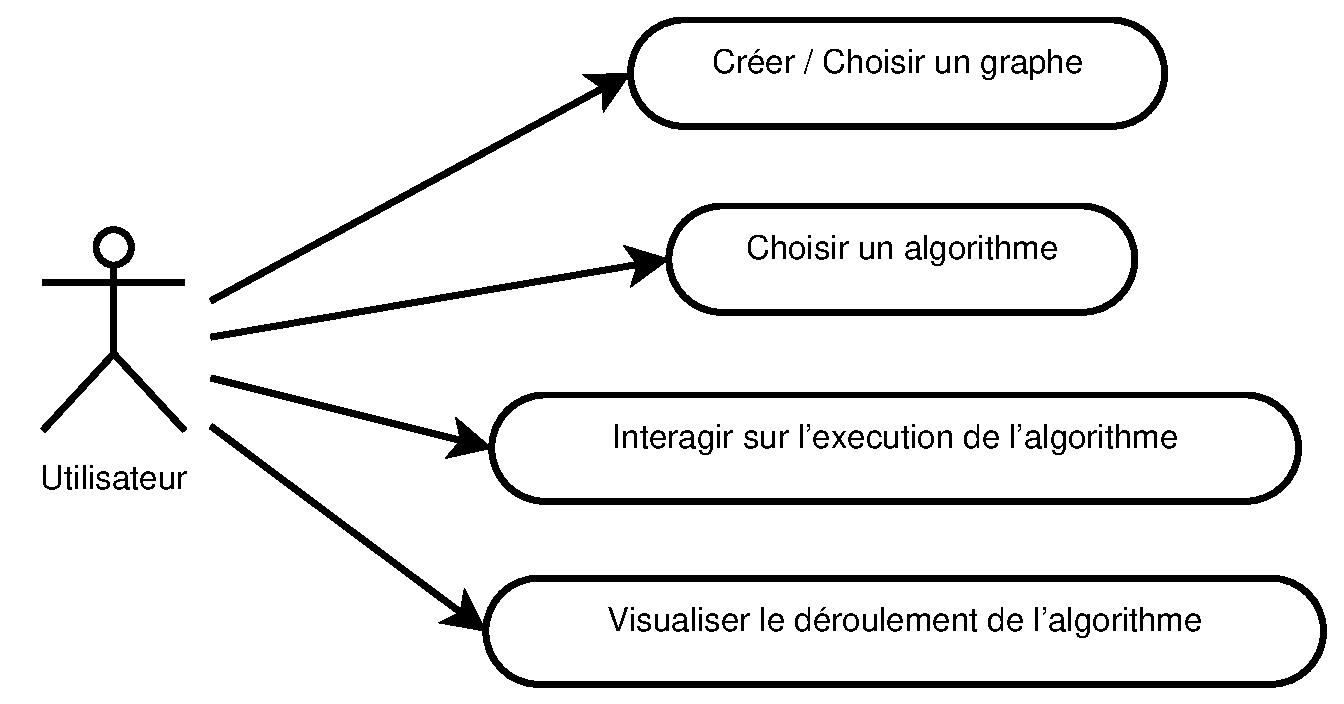
\includegraphics[scale=0.4]{useCase.eps}
					\end{center}
					\caption{Diagramme de Use case}
					\label{img_use_case}
				\end{figure}
				\textbf{Scénario nominal }: L'utilisateur choisit un graphe parmi la liste des graphes disponibles. Le logiciel charge le graphe et affiche à l'écran la visualisation de celui-ci. L'utilisateur choisit un algorithme parmi une bibliothèque d'algorithme puis demande son lancement. A chaque étape importante de l'algorithme, le logiciel affichera l'état du graphe et ainsi l'utilisateur pourra voir le déroulement de l'algorithme et, suivant les algorithmes, pourra l'orienter en choisissant par exemple un sommet.

			\subsubsection{Diagramme de classe}
				\begin{figure}[htbp]
					\begin{center}
						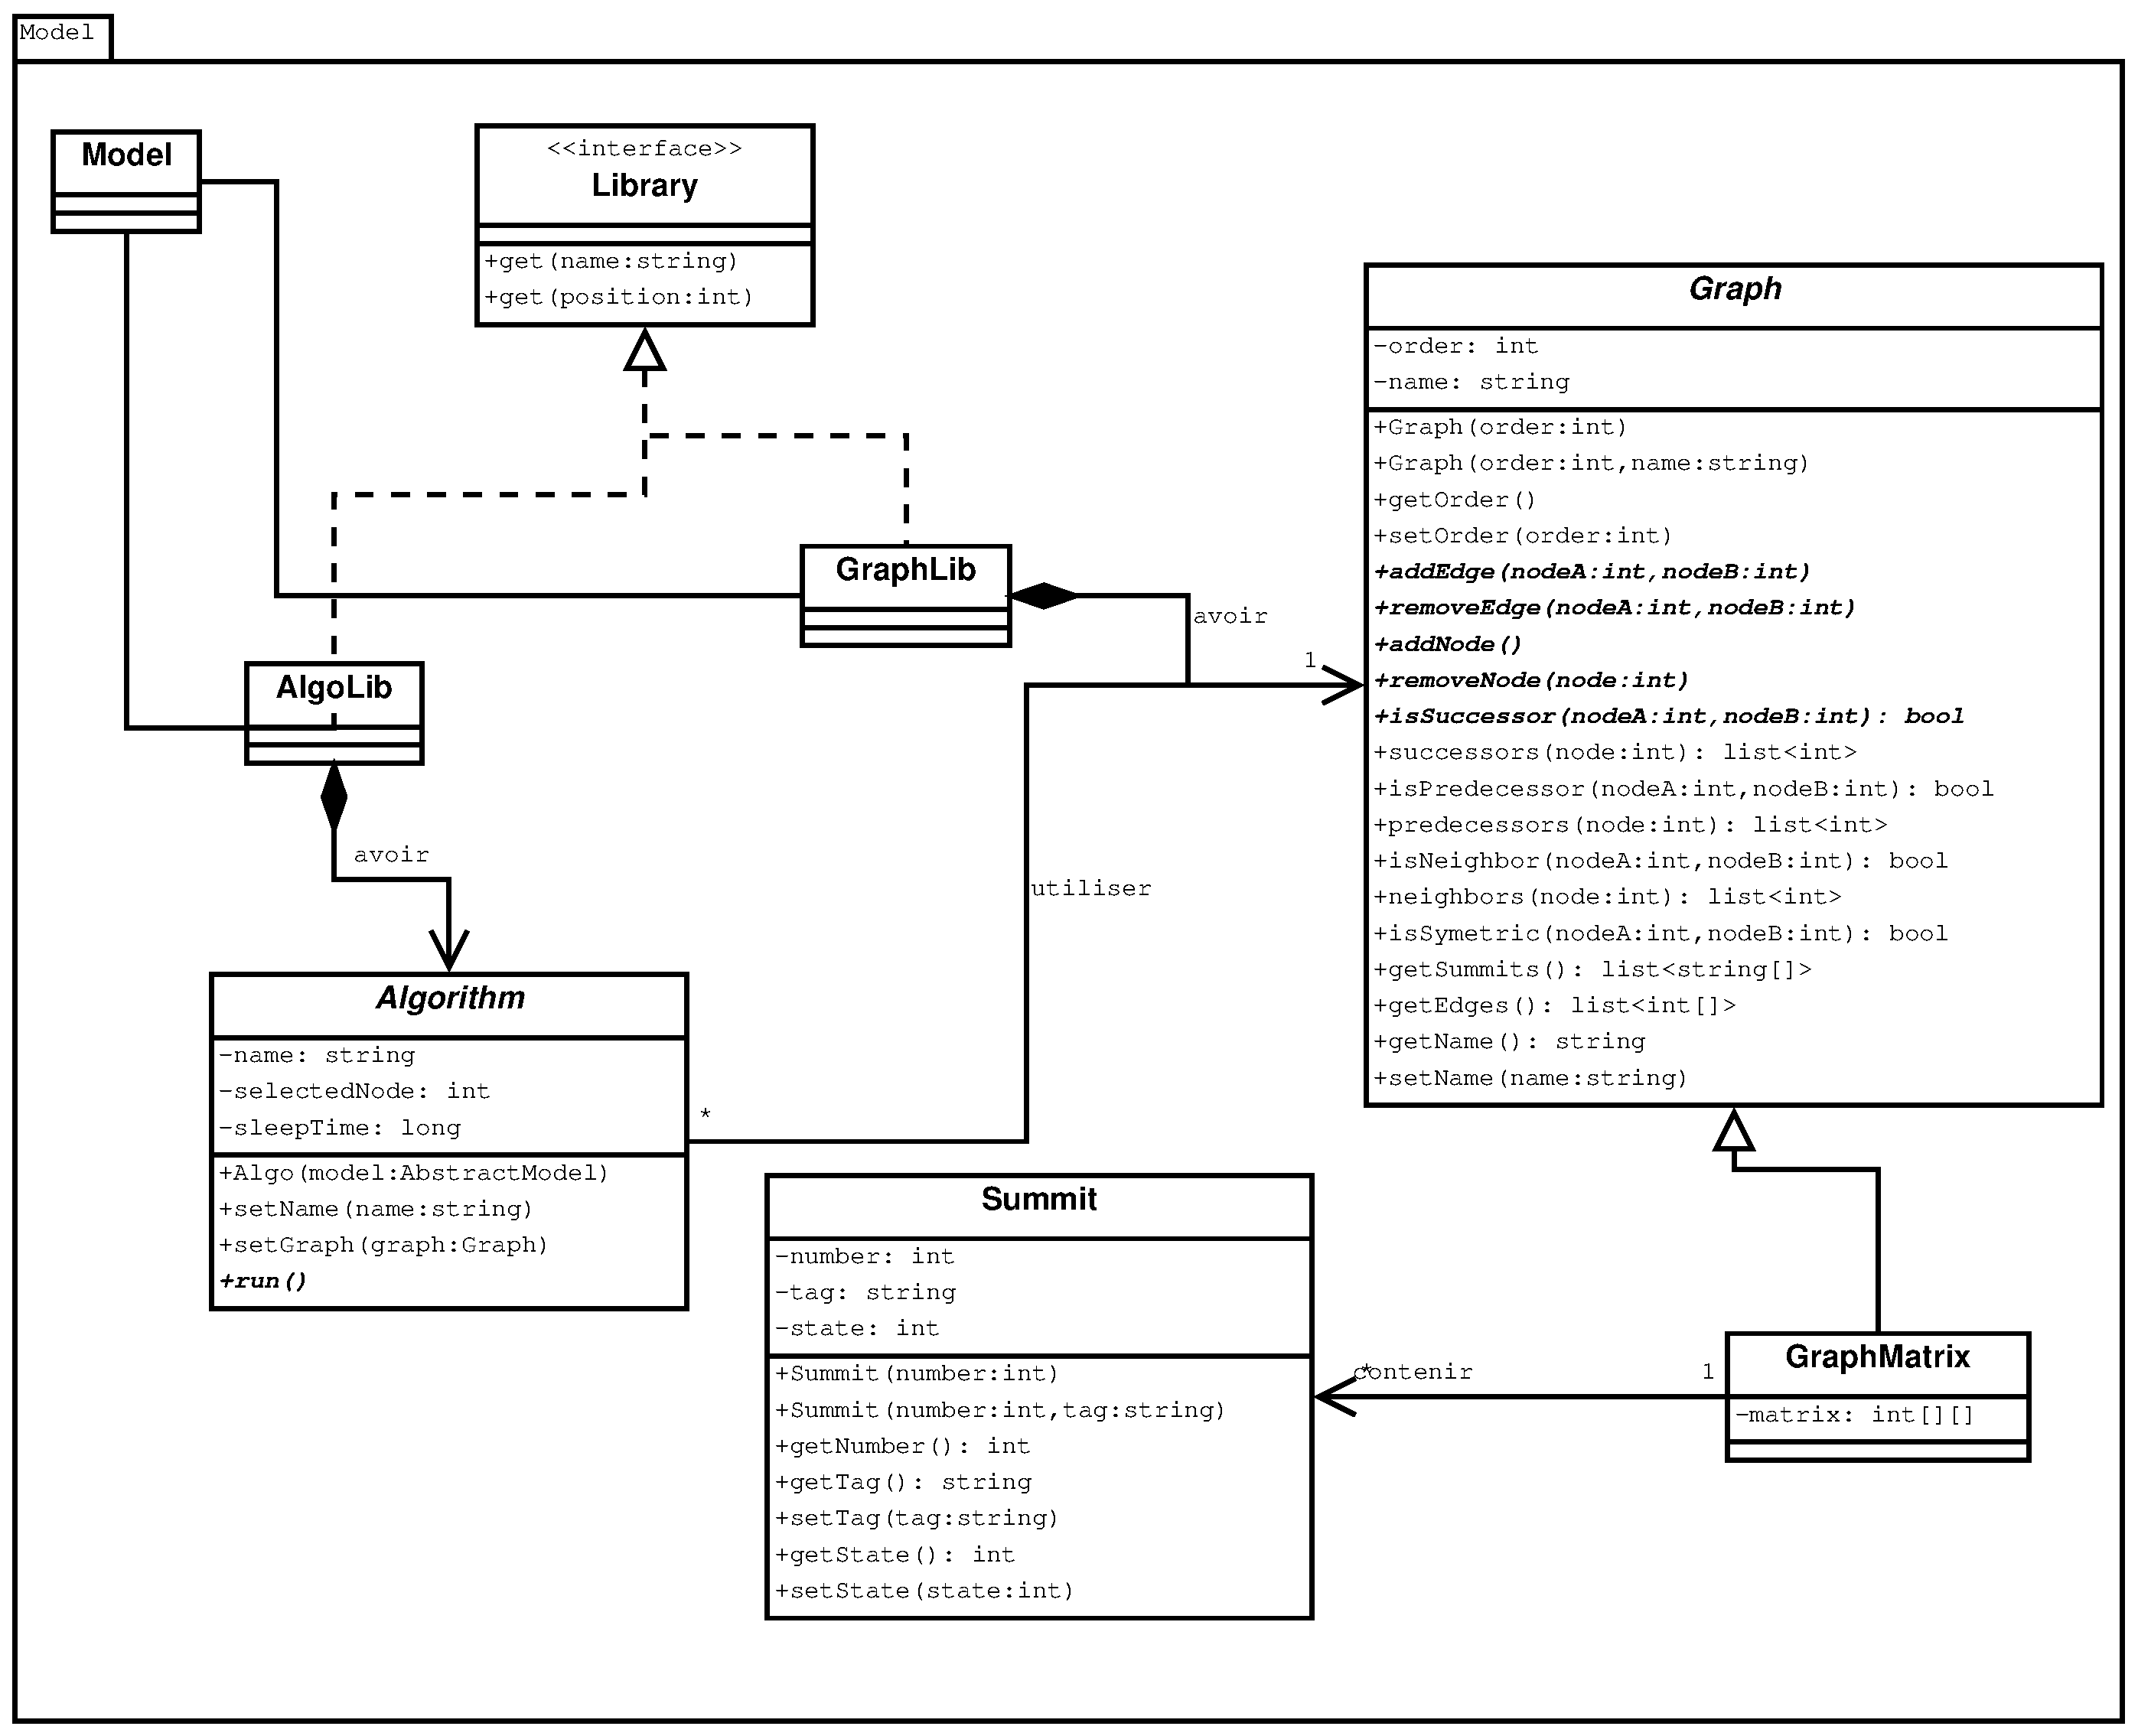
\includegraphics[scale=0.35]{Analyse_class.eps}
					\end{center}
					\caption{Diagramme de classe d'analyse}
					\label{img_class_analyse}
				\end{figure}
		\subsection{Contraintes non fonctionnelles}
			
			Très peu de contraintes non fonctionnelles ont été relevées. En effet, le sujet était assez ouvert, nous n'avions aucune contrainte de technologies, ou bien de plateformes. Les quelques contraintes que nous avons pu recenser sont :
			\begin{itemize}
				\item Le développement du logiciel à l'aide du pattern Modèle Vue Contrôleur (M.V.C.) afin de donner une certaine flexibilité à l'architecture du logiciel.
				\item Le logiciel devra manifester un souci d'ouverture afin de permettre de possibles évolutions.
				\item Après notre premier rendez-vous avec notre tuteur il a été décidé que ce projet sera développé en C++.
			\end{itemize}
			
		\subsection{Outils utilisés}
		
			Afin que le projet se déroule au mieux, divers outils ont été utilisés, qu'ils soient pour l'analyse du projet, son élaboration, ou bien sa gestion.
			Tout d'abord, pour la partie analyse et conception, il a été utile de pouvoir faire différents diagrammes UML, pour cela deux outils ont été utilisé :
			\begin{itemize}
				\item ArgoUML : Logicel libre permettant la création de digramme UML respectant la norme UML1.4. Cet outil permet également la génération de code à partir de diagrammes et ce dans différent langages tels que le C++, le Java, le PHP ...\\
				\textit{http://argouml.tigris.org/}
				\item Dia : Logiciel libre de création de diagrammes de tous types. Il peut également permettre l'édition de diagramme UML, cependant celui-ci est moins abouti qu'ArgoUML, mais en contrepartie, permet des représentations beaucoup plus lisibles des diagrammes réalisés.\\
				\textit{http://live.gnome.org/Dia/}
			\end{itemize} 
						
			~\\Par la suite, pour le développement nous avons utilisé des environnement de développement intégré (I.D.E.) ainsi que des débogueurs : 
			\begin{itemize}
				 \item Eclipse 3.5 Galileo : I.D.E. libre utilisé pour le développement du c\oe ur du logiciel (c'est-à-dire la partie modèle principalement). \\
				 \textit{http://www.eclipse.org/}
				 \item Qt4 : Bibliothèque graphique orientée objet et développée en C++ permettant de concevoir des interfaces graphiques à l'aide de nombreux outils déjà intégrés à la librairie. Cette bibliothèque graphique est très intéressante de part sa portabilité, en effet portable sur des systèmes Unix (Linux et Unix embarqué), Windows Mac OS mais aussi car c'est une bibliothèque qui a été adaptée dans de nombreux langages (C++, Java, Python, C\#). \\
				 \textit{http://qt.nokia.com/}
				 \item QtCreator : I.D.E. développé par Qt Development Frameworks permettant de coder plus aisément des interfaces graphiques se basant sur la bibliothèque graphique Qt. Cet I.D.E. fournit différentes fonctionnalités telles que la création des fenêtres de façon graphique, l'aide associée à la bibliothèque graphique, etc... \\
				 \textit{http://qt.nokia.com/products/appdev/developer-tools}
				 \item Valgrind : Débogueur en mode console permettant de faire du profilage de code et de pouvoir repérer les fuites de mémoires. \\
				 \textit{http://valgrind.org/}
				 \item QtCreator Débogueur : Outils intégré à QtCreator, permettant le débogue d'un programme et plus particulièrement des interfaces graphiques. \\
				 \textit{http://qt.nokia.com/products/appdev/developer-tools}
			\end{itemize}
		
			~\\Enfin, pour l'organisation du projet, nous avions prévu d'utiliser un outil tel qu'une forge gérant le versionnage des fichiers et d'autres fonctionnalités (pour cela nous pensions utiliser Google Code), cependant, suite à quelques soucis dans le binôme (séparation), ces fonctionnalités n'étaient pas nécessaires. 
			Un logiciel permettant la planification de projet a été utilisé, celui-ci nous a permis de bien organiser le projet, ainsi que de se fixer des objectifs à atteindre à des dates données. Le logiciel que nous avons utilisé est, lui aussi, un logiciel libre nommé Planner (\textit{http://www.simpleprojectmanagement.com/planner})

		\subsection{Gestion du projet}
			
			Pour permettre le bon déroulement du projet, nous avons décidé en accord avec notre tuteur de se voir régulièrement pour pouvoir avoir un avis de la part de notre tuteur et donc être le plus proche possible de ce qu'il attendait. Pour cela, nous avons donc décidé de se voir toutes les semaines pendant à peu près une heure. Ces réunions étaient l'occasion de montrer le travail effectué, d'avoir un retour par rapport à cela, et de pouvoir organiser le travail à venir. De plus, cela permettait, d'une part de nous rassurer, mais également de rassurer notre tuteur qui pouvait grâce à cela être au courant de notre avancée.
			
			De plus, un outil de planification a été utilisé, permettant l'organisation du travail en fonction des ressources disponibles et de pouvoir voir l'état du projet au cours du temps et augmenter la priorité de certaines tâches si besoin est (cf Fig. \ref{img_gantt}).
			\begin{figure}[htbp]
				\begin{center}
					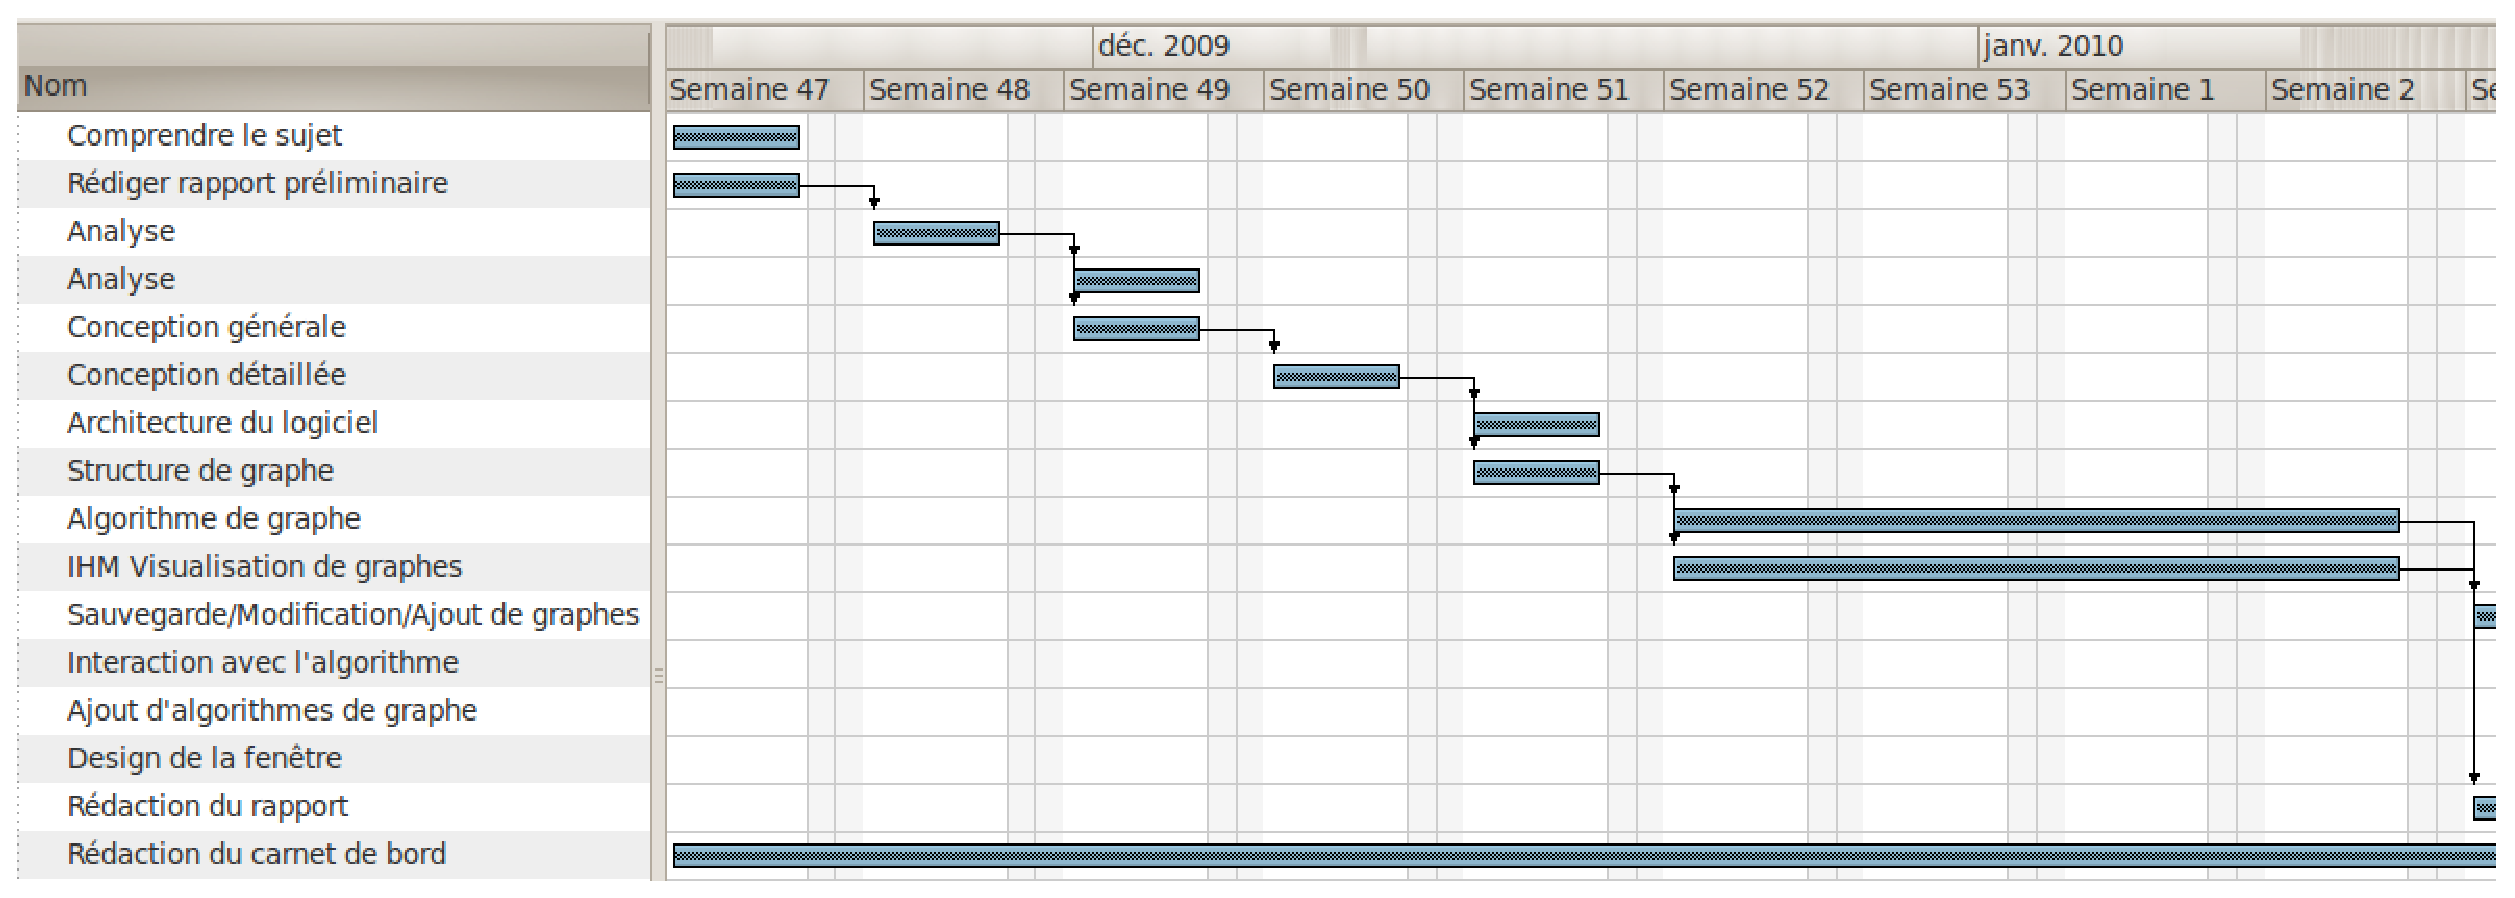
\includegraphics[scale=.4]{gantt.eps}
					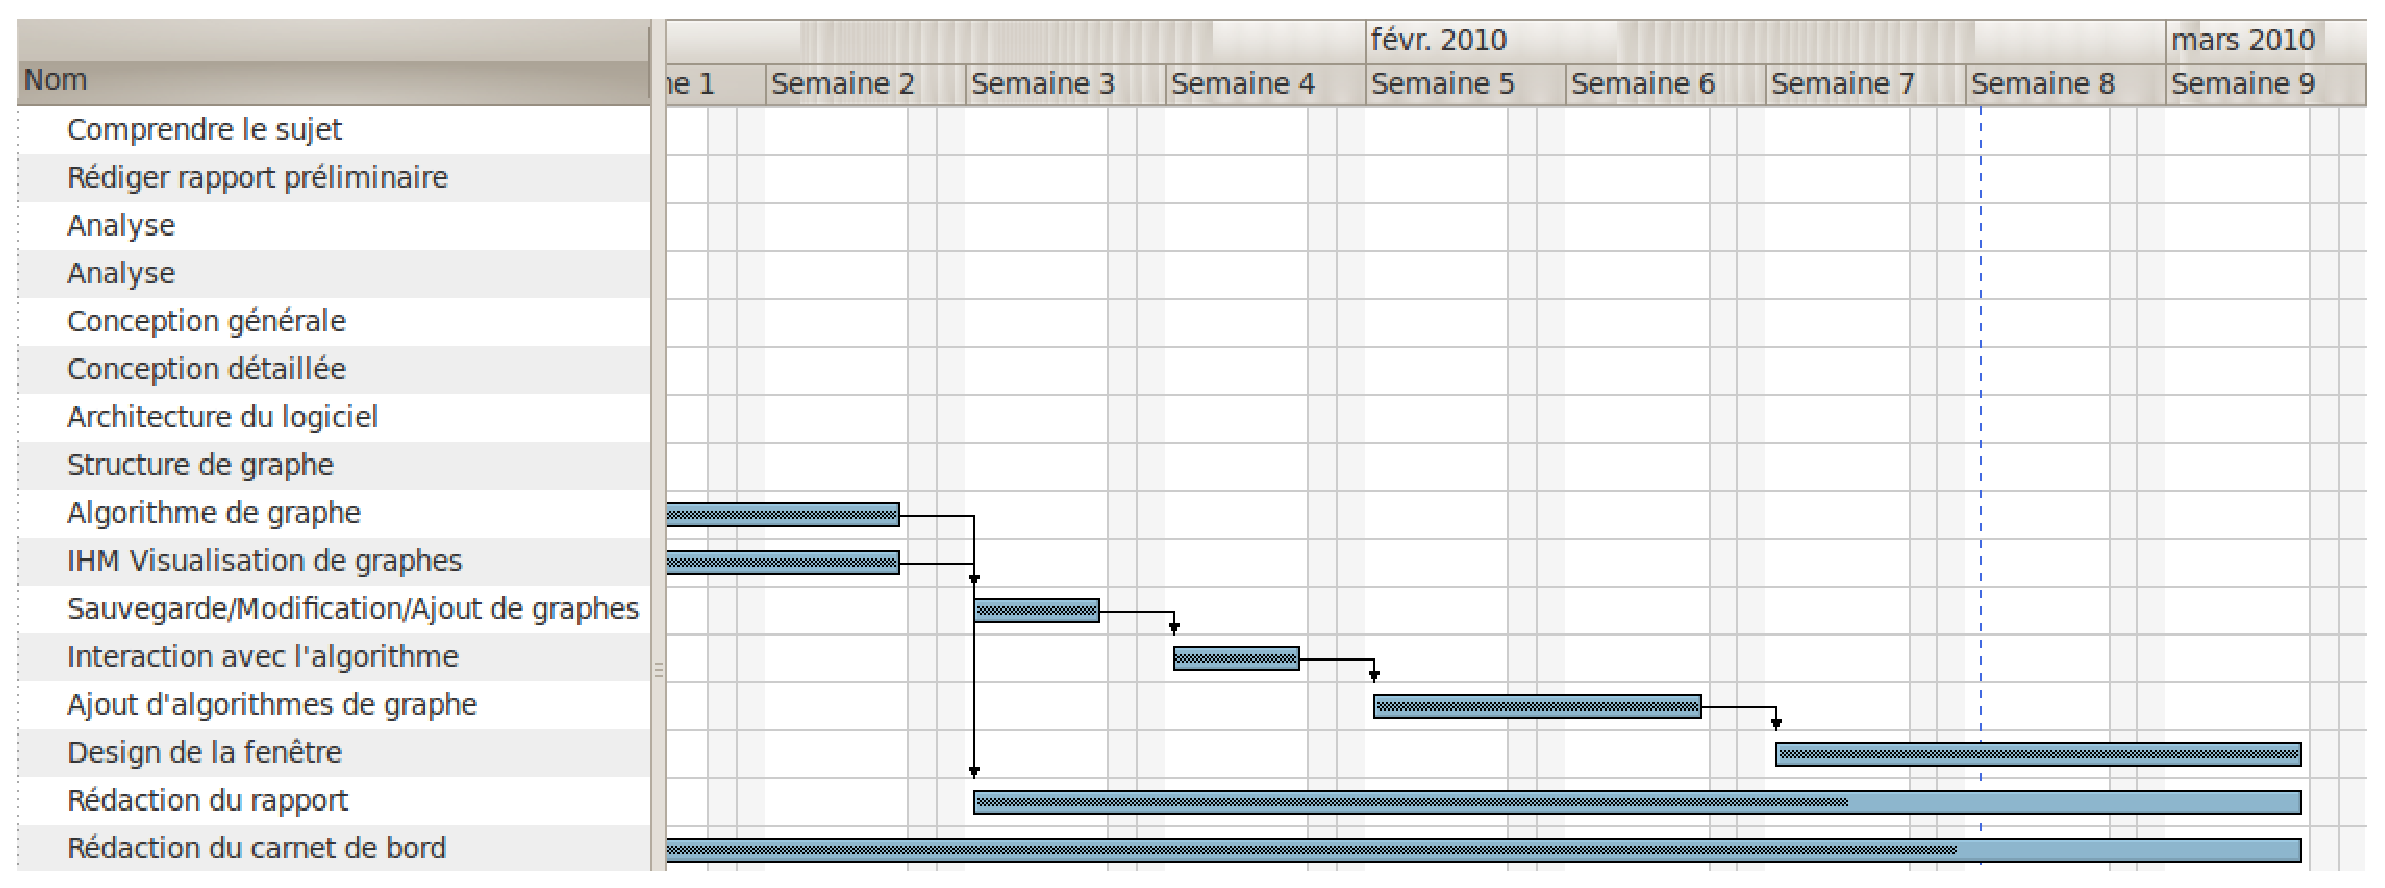
\includegraphics[scale=.4]{gantt2.eps}					
				\end{center}
				\caption{Planning réalisé pour le déroulement du projet}
				\label{img_gantt}
			\end{figure}
	
	\newpage
	\section{Conception}
	
		Afin de bien organiser le développement du logiciel nous avons dû séparer les différents composants du logiciel et établir une architecture basée sur le M.V.C. Pour ce faire, nous avons donc amélioré notre premier diagramme de classe pour créer l'architecture du logiciel.
		\subsection{Diagramme de classe}
			\begin{figure}[htbp]
				\begin{center}
					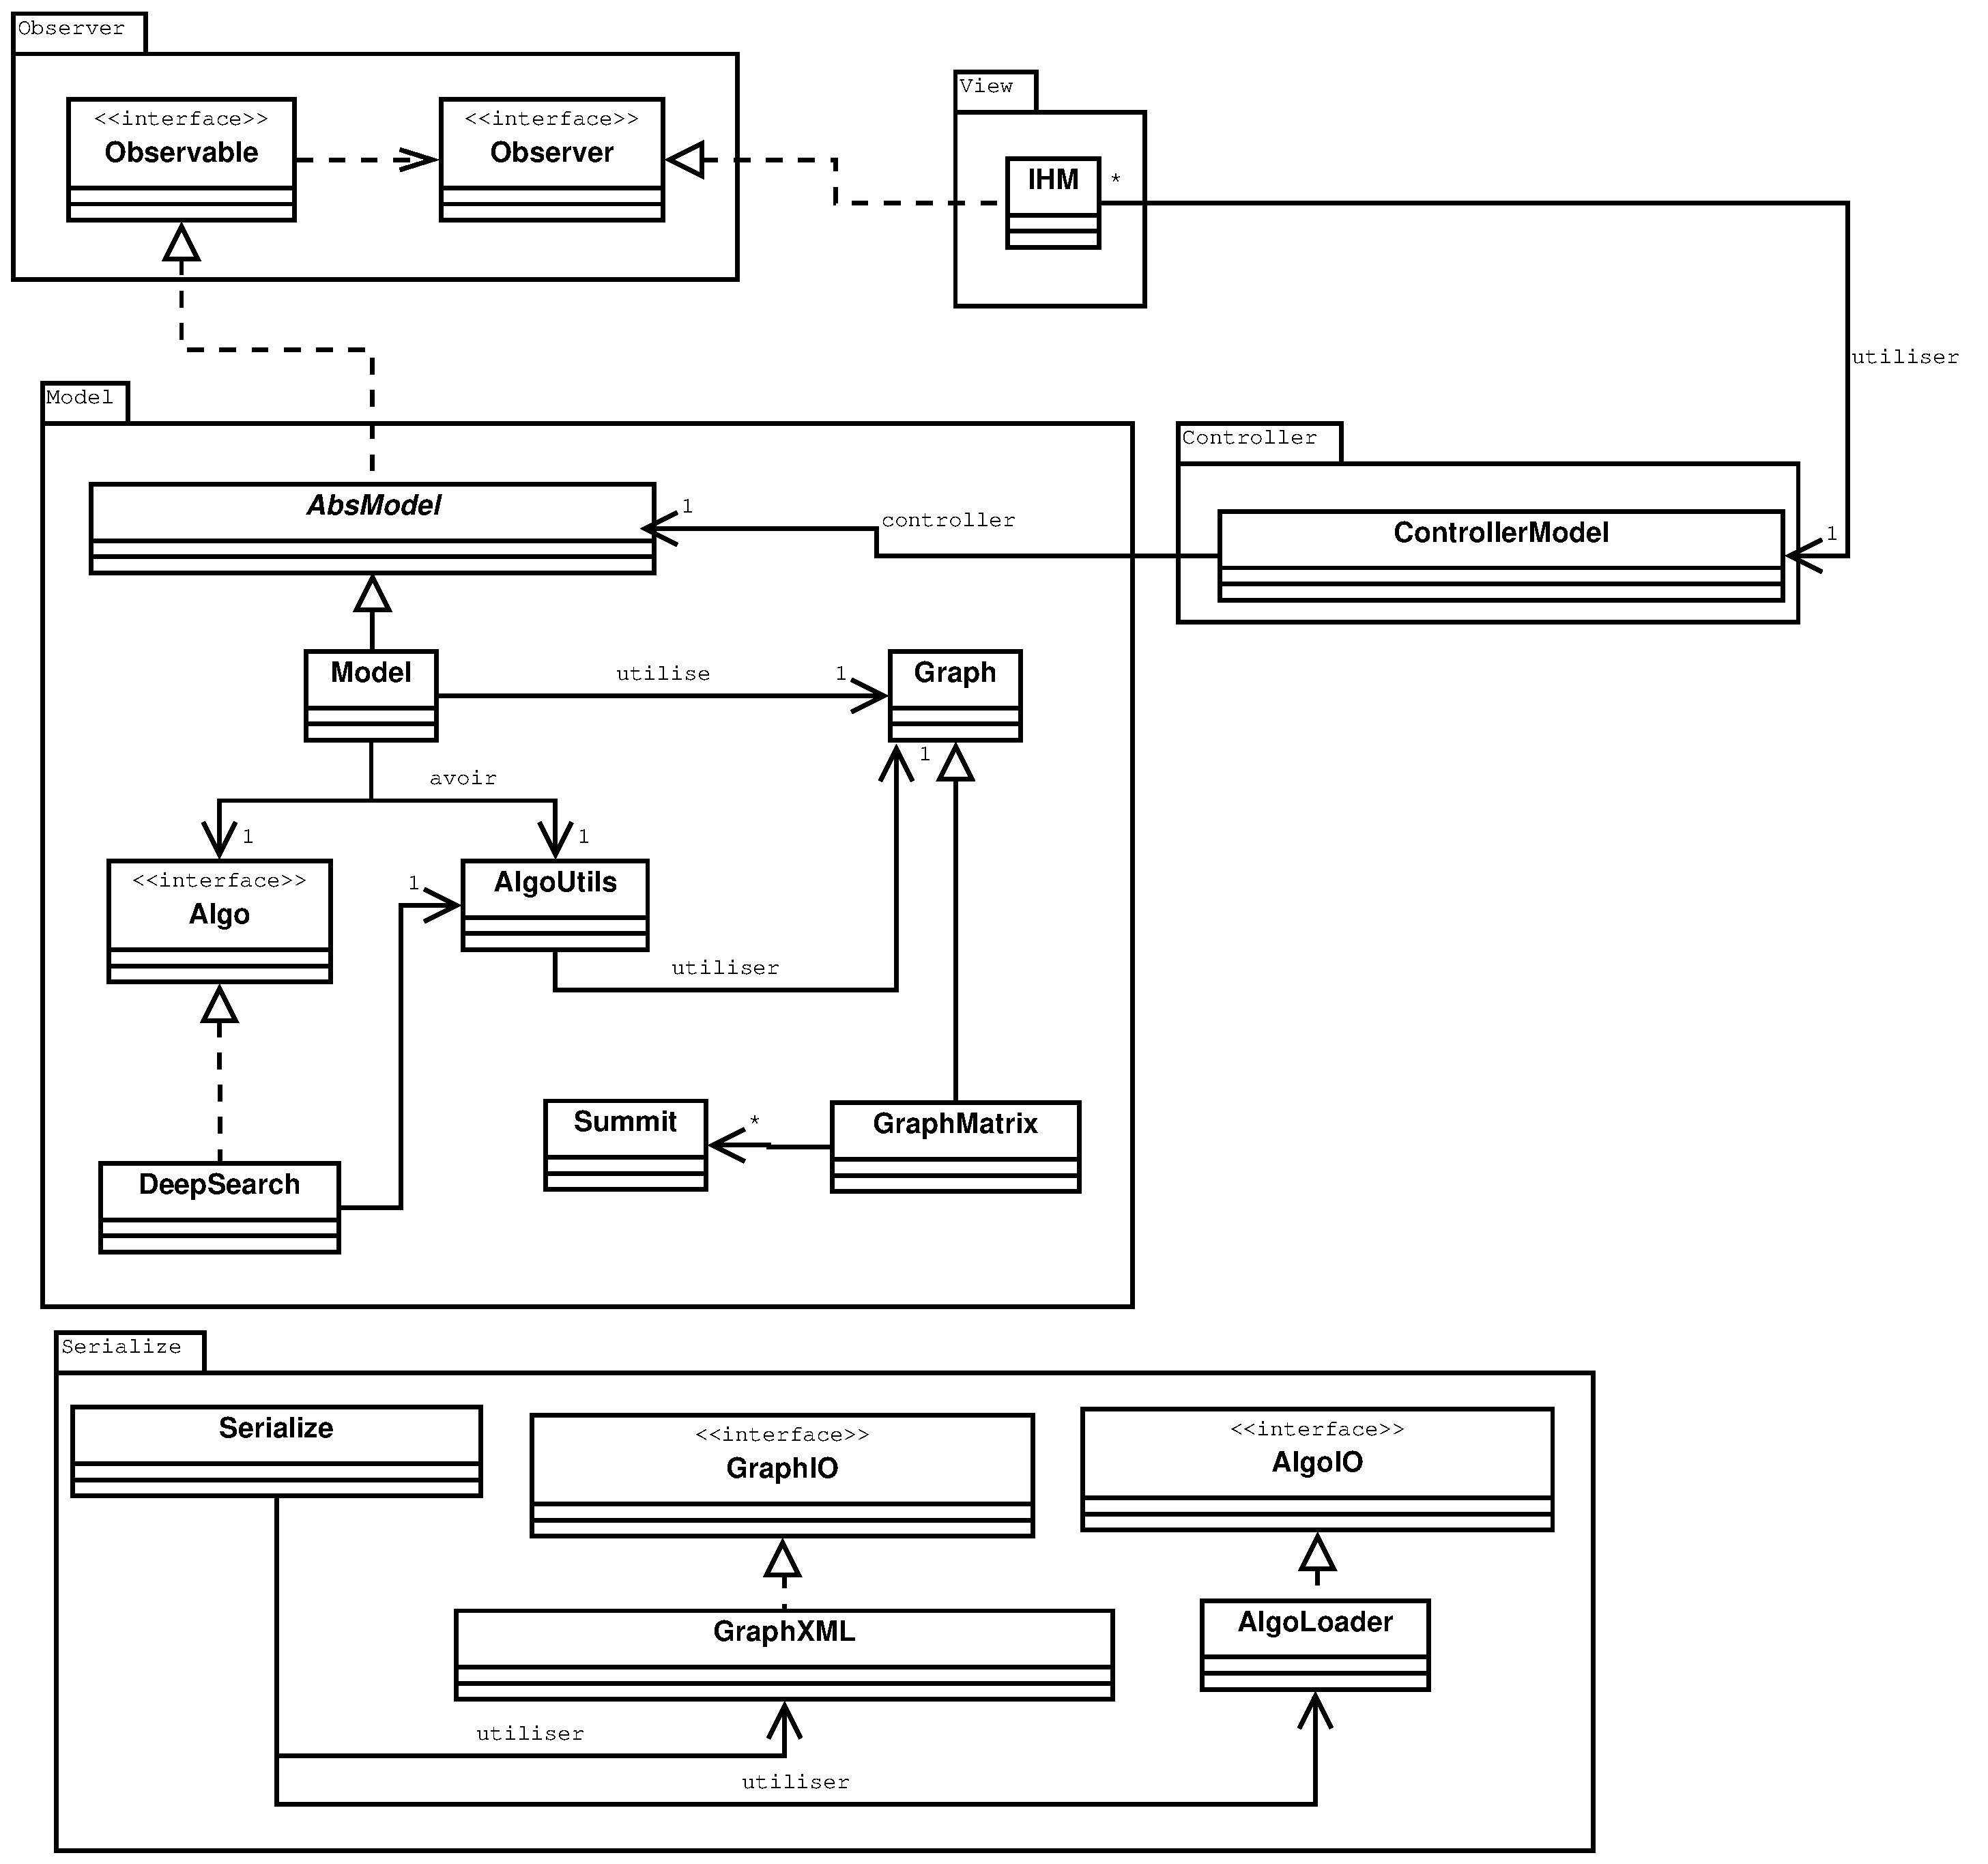
\includegraphics[scale=0.30]{class_esquisse.eps}
				\end{center}
				\caption{Diagramme de classe de conception (mode esquisse)}
				\label{img_class_esquisse}
			\end{figure}
			Diagramme de classe en mode plan fourni en annexe (Fig. \ref{img_class_model}, \ref{img_class_serialize}, \ref{img_class_controler}, \ref{img_class_observer}, \ref{img_class_ihm})
				
		\newpage
		\subsection{Diagramme de package}
			\begin{figure}[htbp]
				\begin{center}
					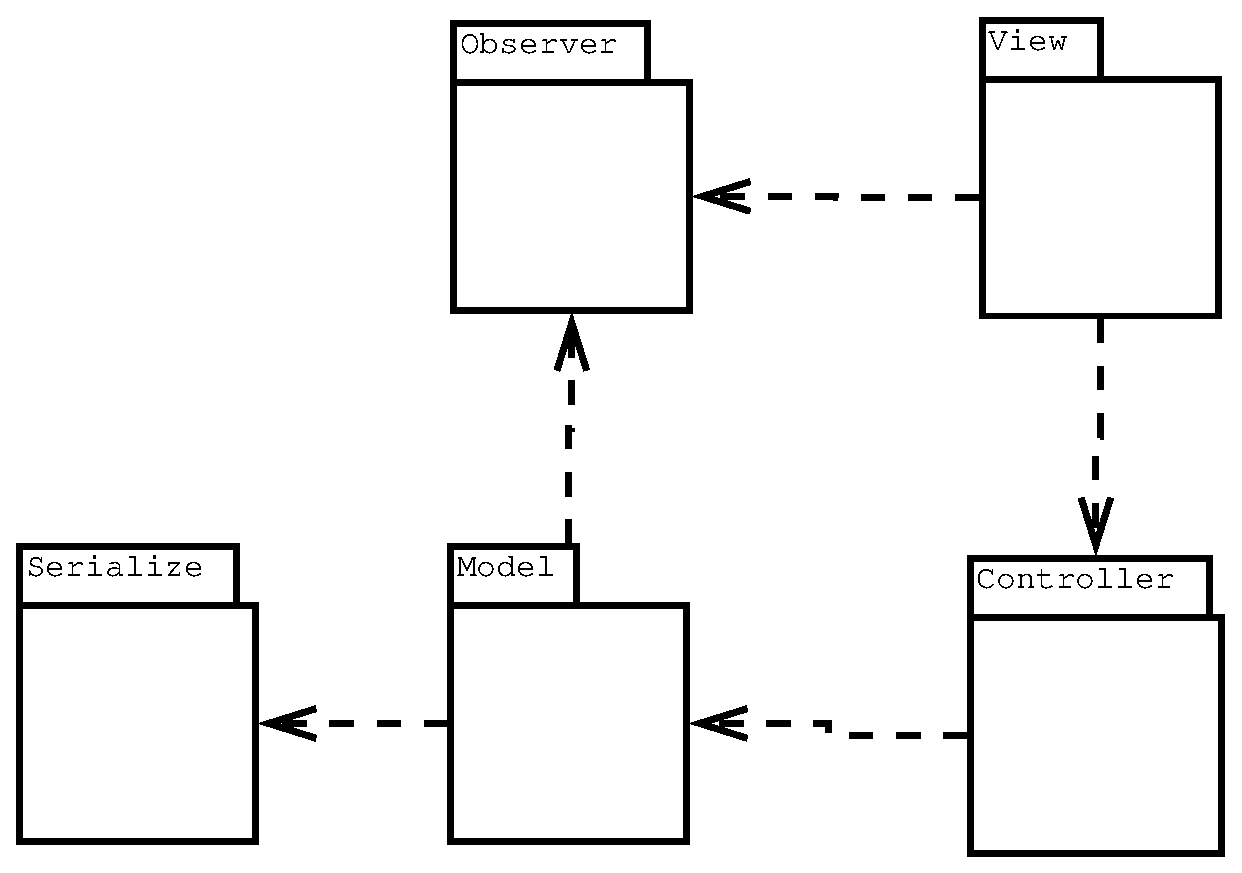
\includegraphics[scale=0.5]{packages.eps}
				\end{center}
				\caption{Diagramme de package}
				\label{img_package}
			\end{figure}
			A l'aide de ce diagramme de package, on voit bien l'avantage du M.V.C, en effet, on se rend compte que la vue est totalement indépendante du modèle. Ceci peut donc s'avérer utile si on décide de changer d'interface graphique par exemple. Ceci est notamment utile si des ajouts ou des modifications sont effectuées sur le modèle. Il est donc possible d'ajouter des structures de graphes ou des algorithmes sans avoir à modifier quoi que ce soit sur notre interface graphique, et inversement, on peut modifier notre interface sans avoir à modifier notre modèle. Grâce à cela, on a donc un logiciel qui peut assez facilement évoluer sans avoir à retoucher tout le programme.
	
	\newpage
	\section{L'objet Graphe}
		\begin{figure}[htbp]
			\begin{center}
				\includegraphics[scale=0.3]{class_graph.eps}
			\end{center}
			\caption{Classe Graph}
			\label{img_graph_class}
		\end{figure}
		
		\subsection{Sauvegarde et importation}
			Dans le cahier des charges, il était stipulé que les graphes devraient pouvoir être sauvegardés. Pour ce faire, nous avons décidé d'effectuer la sauvegarde dans un fichier XML. En effet, la sérialisation XML est beaucoup utilisée que ce soit dans les logiciels (sauvegarde de données, propriétés liées au programme) ou bien les services web ou les technologies web. De plus, la sérialisation XML s'avère assez aisée à utiliser.
			Après quelques recherches concernant des parser XML en C++, nous avons découvert TinyXML (parseur XML libre et open source) qui s'avérait relativement simple à utiliser, s'appuyant sur la technologie DOM qui crée un arbre contenant l'ensemble du fichier XML. Grâce à cela, il est donc possible de naviguer dans l'arbre en parcourant les enfants d'un sommet. Nous avons donc défini une structure pour la sauvegarde d'un graphe qui est la suivante : \\\\
			\begin{tabular}{|l|}
				\hline 
				$<$graph name=""$>$ \\
 					\indent$<$order$><$/order$>$ \\
					\indent$<$listNode$>$ \\
						\indent\indent$<$node num="" tag="" state=""/$>$ \\
						\indent\indent...\\
					\indent$<$/listNode$>$\\
					\indent$<$listEdge$>$\\
						\indent\indent$<$edge start="" end="" value="" state=""/$>$\\
						\indent\indent...\\
					\indent$<$/listEdge$>$\\
				$<$/graph$>$\\
				\hline 
			\end{tabular}  
			\\\\
		Grâce à cette structure, il nous est maintenant possible de sauvegarder un graphe, mais pas uniquement l'ensemble de ses n\oe uds et de ses arcs, mais également l'état de ceux-ci ainsi que leurs valeurs. A partir de cela, il est donc possible de restaurer un graphe avec l'état de chacun de ses n\oe uds et de ses arcs.	
			
		\subsection{Structure de graphe utilisée}
			Le logiciel devait permettre l'ajout de nouvelles structures de graphe. A l'heure actuelle, seule la structure de graphe symbolisée par une matrice a été implémentée. D'autres structures sont possibles, en effet, un graphe peut se représenter en machine à l'aide de différentes structures comme : 
			\begin{itemize}
				\item \textbf{Représentation par le biais d'une matrice} : Une matrice de contenant $n * n$ cases avec $n$ étant l'ordre du graphe, et où chaque case $i$, $j$ (avec $i,j \in 0..n$) contient une valeur booléenne permettant de savoir s'il y a oui ou non un arc entre le n\oe ud $i$ et le n\oe ud $j$.
				\item \textbf{Représentation par le biais d'un tableau de liste de successeurs} : Dans cette représentation nous avons un tableau de taille $n$, avec $n$ étant l'ordre du graphe, et chaque case $i$ (avec $i \in 0..n$) contient l'ensemble des successeurs de $i$.
				\item \textbf{Représentation par une liste d'arcs} : Cette représentation est la moins utilisée des trois, elle contient uniquement un entier $n$ représentant le nombre de n\oe uds du graphe, et une liste contenant les arcs du graphe.
			\end{itemize}
			
			Bien entendu, ces structures sont simplifiées et différentes implémentations sont possibles suivant les besoins de chacun. 
			
			Pour ce projet nous avons donc utilisé une structure représentée par une matrice, cependant des modifications ont été effectuées. En effet, notre matrice ne contient pas simplement une valeur permettant de savoir si oui ou non il y a un arc, dans notre cas, chaque case $i$, $j$ contient un entier négatif s'il n'y a pas d'arc entre $i$ et $j$ et un entier supérieur à 0 s'il y a un arc, et cette valeur correspond à la valeur de l'arc. De plus en se basant sur le même principe, nous avons une deuxième matrice qui nous permet de sauvegarder l'état des arcs et enfin nous avons une liste d'objets représentant un n\oe ud, dans lesquels sont enregistrés l'état et l'étiquette de chaque n\oe ud. 
			
		\subsection{Ajout de structures de graphe}
			Grâce à la structure du logiciel, il est possible d'ajouter de nouvelles structures de graphe basées sur celles décrite précédemment ou éventuellement de nouvelles structures issu de réflexions diverses et variées. Pour ce faire, il suffit de faire hériter notre nouvelle structure de la classe Graph (cf Fig. \ref{img_graph_class}). Cette classe contient différentes méthodes dont certaines abstraites qu'il faudra donc redéfinir dans notre nouvelle structure. Ces méthodes à redéfinir sont les suivantes : 
			\begin{itemize}
				\item \textit{void addEdge(int nodeA, int nodeB)} : Ajoute un arc reliant le n\oe ud $nodeA$ au n\oe ud $nodeB$ avec $nodeA, nodeB \in 0..n$.
				\item \textit{void removeEdge(int nodeA, int nodeB)} : Supprime l'arc reliant $nodeA$ à $nodeB$ avec $nodeA, nodeB \in 0..n$.
				\item \textit{void addNode()} : Ajoute un n\oe ud au graphe.
				\item \textit{void removeNode(int node)} : Supprime le n\oe ud node du graphe avec $node \in 0..n$.
				\item \textit{bool isSuccessor(int nodeA, int nodeB)} : Retourne vrai si le $nodeA$ est un successeur de $nodeB$, faux sinon avec $nodeA, nodeB \in 0..n$.
				\item \textit{int getEdgeValue(int nodeA, int nodeB)} : Retourne la valeur de l'arc $nodeA, nodeB$ avec $nodeA, nodeB \in 0..n$.
				\item \textit{void setEdgeValue(int nodeA, int nodeB, int value)} : Assigne la valeur $value$ à l'arc $nodeA, nodeB$ avec $nodeA, nodeB \in 0..n$.
				\item \textit{int getEdgeState(int nodeA, int nodeB)} : Retourne l'état de l'arc $nodeA, nodeB$ avec $nodeA, nodeB \in 0..n$.
				\item \textit{void setEdgeState(int nodeA, int nodeB, int state)} : Assigne l'état $state$ à l'arc $nodeA, nodeB$ avec $nodeA, nodeB \in 0..n$ et $state \in 0..3$.
			\end{itemize}
			\vspace*{.5cm}
			\indent\indent D'autres fonctions peuvent être redéfinies, cela n'est pas nécessaire, mais peut s'avérer utile lorsque de bonnes performances sont attendues ou simplement lorsque l'on en a envie. Une fois toutes les fonctions utiles redéfinies, la structure peut être utilisée avec n'importe quel algorithme.
			
	\newpage
	\section{L'objet Algorithme}
		\begin{figure}[htbp]
			\begin{center}
				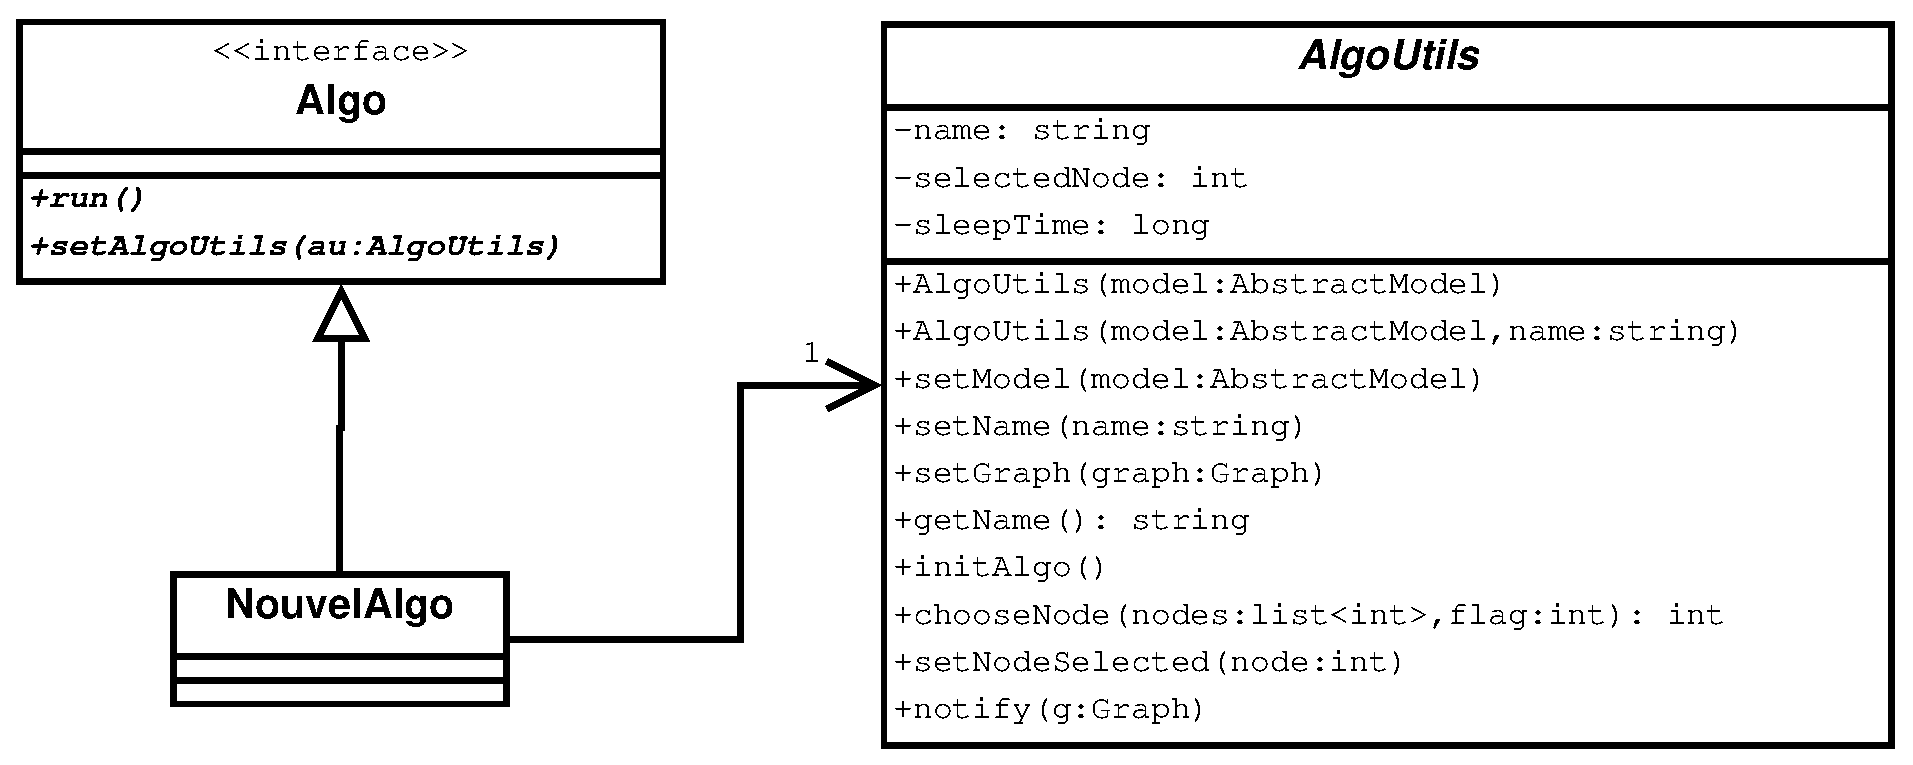
\includegraphics[scale=0.5]{class_algo.eps}
			\end{center}
			\caption{Classe Algo}
			\label{img_algo_class}
		\end{figure}	
				
		\subsection{Ajout d'algorithmes}
			Ce logiciel offre la possibilité d'y intégrer ses propres algorithmes. Afin que ceux-ci soient correctement utilisables, certaines contraintes sont à respecter. Dans un premier temps, comme on peut le voir sur le diagramme UML (Fig. \ref{img_algo_class}), notre algorithme doit hériter de l'objet algo et doit de ce fait, redéfinir les fonctions \textit{run(g:Graph)} et \textit{setAlgoUtils(au:AlgoUtils}) qui sont respectivement les fonctions permettant de lancer l'algorithme sur le graphe $g$ fourni en paramètre et la fonction permettant d'attribuer à notre algorithme quelques fonctions utiles, comme la fonction chooseNode() qui retourne un n\oe ud choisi par l'utilisateur parmi une liste de n\oe uds fournie par l'algorithme. En plus de ces fonctions à implémenter et de l'héritage à faire, il est également nécessaire de rajouter un créateur et un destructeur externe à l'objet, ce qui sera utile lors du chargement de l'algorithme (cf Chargement dynamique des algorithmes). Ce créateur appelé \textit{create} et retournant un objet Algo va avoir pour but de créer le nouvel algorithme (l'équivalent d'un new NouvelAlgo()). De même, pour le destructeur appelé \textit{destroy} avec comme paramètre un objet Algo, permet de détruire l'algorithme lorsque nous n'en avons plus besoin.
			
			Après tout cela, notre nouvel algorithme s'organise donc de la manière suivante : 
			
			\begin{tabular}{|l||l|}
				\hline 
				NouvelAlgo.h 								& NouvelAlgo.cpp\\
				\hline
				$\sharp$ ifndef NOUVELALGO\_H 				& $\sharp$ include "NouvelAlgo.h"\\
				$\sharp$ define NOUVELALGO\_H 				& NouvelAlgo::NouvelAlgo()$\lbrace \rbrace$\\
				$\sharp$ include "Algo.h"					& NouvelAlgo::~NouvelAlgo() $\lbrace \rbrace$\\
				class NouvelAlgo : public Algo $\lbrace$ 	& void NouvelAlgo::run(Graph *g) $\lbrace \rbrace$\\
				public: 									& void NouvelAlgo::setAlgoUtils(AlgoUtils *au) $\lbrace $\\
				\indent NouvelAlgo(); 						& \indent this$\rightarrow$au = au;\\
				\indent virtual ~NouvelAlgo(); 				& $\rbrace$\\
				\indent run(Graph $*$g); 					& extern "C" Algo* create()$\lbrace$ \\
				\indent setAlgoUtils(AlgoUtils $*$au);		& \indent return new NouvelAlgo;\\
				private:									& $\rbrace$\\
				\indent AlgoUtils $*$au; 					& extern "C" void destroy(Algo* a) $\lbrace$ \\		
				$\rbrace$ ; 								& \indent delete a;\\
				$\sharp$endif 								& $\rbrace$\\		
				\hline 
			\end{tabular} 
			~\\~\\
			Libre à vous par la suite de créer de nouvelles fonctions ou attributs à l'intérieur de l'algorithme ne servant qu'à celui-ci.
			
			Ces fichiers doivent être placés dans le répertoire model/Algorithm du projet afin que les dépendances soient satisfaites.

		\subsection{Chargement dynamique des algorithmes}
			L'une des principales contraintes de ce logiciel était de le faire évolutif. Pour cela, nous avons permis l'ajout d'algorithme (voir chapitre précédent). Pour ne pas avoir à recompiler à chaque fois l'ensemble du logiciel pour l'ajout d'un algorithme nous voulions faire ceci à la manière de greffon. En effet, chaque algorithme sera un greffon de notre logiciel, et nous pourrons donc ajouter de nouveaux greffons facilement sans avoir à effectuer des modifications sur le logiciel. Tout se fera automatiquement et nous aurons seulement à ajouter le fichier source de notre algorithme ou bien la librairie (.so sous linux et .dll sous windows).
			
			Cette partie a été la plus difficile à réaliser car si cela est plutôt simple à réaliser en Java (deux lignes suffisent), cela se complexifie en C++. Après de multiples recherches nous avons remarqué que l'héritage était très mal géré, c'est pour cela que nous avons dû dissocier l'objet Algo et l'objet AlgoUtils qui étaient, dans un premier temps, un seul et même objet. Grâce à cette modification, nous avons pu charger nos algorithmes grâce à la librairie \textit{dlfcn.h} sous système Unix et windows.h sous système Windows. Ces librairies permettent de charger une librairie partagée grâce à la fonction \textit{dlopen()} (\textit{LoadLibrary()} sous Windows). Une fois cette librairie chargée, les fonctions de l'algorithme sont récupérées grâce à la fonction \textit{dlsym()} (\textit{GetProcAddress()} sous Windows) qui récupère un pointeur sur une fonction déclarée externe à l'objet. C'est pour cela que lors de la création d'un nouvel algorithme, il est nécessaire d'avoir nos fonctions \textit{create()} et \textit{destroy()} qui sont externes, cela permet de créer l'objet afin de l'utiliser par la suite, et pouvoir le détruire après. Et enfin il ne faut pas oublier de fermer la librairie que nous venons d'ouvrir à l'aide de la fonction \textit{dlclose()} (\textit{FreeLibrary()} sous Windows). Grâce à ces fonctions, nous pouvons charger nos nouveaux algorithmes sans que l'ajout de ceux-ci nécessite une recompilation du logiciel tout entier. Nous pouvons donc maintenant simplement ajouter un algorithme par le biais de l'interface graphique très facilement. Il suffit pour cela de créer notre source de l'algorithme en suivant les contraintes vues dans le paragraphe précédent et de l'ajouter, par le biais de l'interface graphique qui fera le travail de compilation en librairie dynamique et le chargera dans l'interface graphique. Celui-ci sera donc utilisable sans même avoir à redémarrer le logiciel. 
		
		\subsection{Algorithmes implémentés}
			Afin de fournir une version que l'on puisse utiliser, le logiciel devait être fourni avec une bibliothèque d'algorithmes. Pour ce faire, nous avons donc développé deux algorithmes. Ces algorithmes ont été choisis car ce sont des algorithmes enseignés lors de l'apprentissage des graphes. En effet, cette année, pour nous familiariser avec les graphes, nous avons analysé ces algorithmes. Ces algorithmes ne présentent pas de grosses difficultés et il est relativement simple de pouvoir faire la trace de ceux-ci en utilisant des petits exemples.
			\subsubsection{Descente en profondeur}
				Premièrement, nous avons développé une descente en profondeur. Cet algorithme permet de connaître tous les descendants d'un n\oe ud, c'est-à-dire, de manière plus vulgarisé, l'ensemble des points vers lesquels on peut aller en suivant les flèches. Ce type d'algorithme peut être utile dans de multiples cas. Si on prend comme exemple un réseau de communication, la descente du graphe permettra de conna\^itre les points vers lesquels on peut communiquer.
				
				Cet algorithme de descente peut être implémenté en suivant diverses méthodes et de diverses façons. Tout d'abord, deux méthodes s'offrent à nous : 
				\begin{itemize}
					\item Depth-first search (Recherche en profondeur) : Cet algorithme va parcourir le graphe en allant le plus loin possible et en remontant pour explorer les nouvelles branches pas encore parcourues.
					\item Breadth-First Search (Recherche en largeur) : Ici, l'algorithme va lister les n\oe uds vers lesquels il peut aller pour ensuite les parcourir un par un.
				\end{itemize}
				Pour implémenter cet algorithme, nous avons décidé de faire une descente en profondeur dont vous pouvez voir l'algorithme ci dessous.
				
				\begin{algorithm}[htpb]
					Descente\_en\_profondeur(entier $n$)\\
					\Donnees{Un n\oe ud $n$ appartenant au graphe $g$}
					\Res{Un ensemble contenant les descendants de $n$ appartenant au graphe $g$}
					\Deb{			
						\PourCh{successeurs $succ$ de $n$ dans $g$}{
							\Si{$succ$ non marqué}{
								sauvegarde du descendant $succ$\\
								marquer $succ$ dans $g$\\
								Descente\_en\_profondeur($succ$)
							}
						}
					}
					\caption{Algorithme de descente en profondeur}
				\end{algorithm}
				
			\subsubsection{Tri topologique}
				Le deuxième algorithme implémenté est celui du tri topologique, également appelé numérotation compatible. Cet algorithme permet de parcourir le graphe de manière à ce qu'un sommet soit toujours parcouru avant ses successeurs. Afin de parcourir l'ensemble des n\oe uds du graphe, il est nécessaire que celui-ci soit acyclique, c'est-à-dire qui ne contienne pas de cycle et donc qu'on ne puisse pas, à partir d'un n\oe ud du graphe, revenir à ce n\oe ud. Cependant, si nous avons un tel graphe $G$ contenant un ou plusieurs cycles, l'algorithme fonctionnera mais parcourra uniquement les n\oe uds du sous graphe acyclique de $G$.
				
				Un tel algorithme peut avoir différentes utilités. Par exemple, nous avons une liste de tâche à effectuer et certaines tâches doivent être effectuées dans la continuité d'autres tâches pour leur bon déroulement. Si nous utilisons un graphe où un n\oe ud représente une tâche et un arc représente la dépendance entre deux tâches, cet algorithme permettra de savoir par quelle(s) tâche(s) nous pouvons commencer et l'enchaînement des tâches suivantes.
				
				Vous pouvez voir cet algorithme ci dessous.
				\begin{algorithm}[htpb]
					Tri\_topologique()\\
					\Donnees{Un graphe $g$}
					\Res{La numérotation compatible de $g$}
					\Deb{
						$i = 0$\\
						copier le graphe $g$ dans $g'$\\		
						\Tq{il reste des sources dans $g'$}{
							choisir une source $src$ de $g'$\\
							val($src$ dans $g$) = $i$\\
							supprimer $src$ de $g'$\\
							$i++$
						}
					}
					\caption{Algorithme de tri topologique}
				\end{algorithm}
			
			\vspace*{5cm}			
	\newpage
	\section{Interface graphique}
		\subsection{Représentation d'un graphe}
			Afin de pouvoir bien visualiser un graphe, nous ne pouvions pas nous contenter de simplement afficher les n\oe uds sans leur affecter de positions précises permettant de ne pas surcharger la représentation. Dans un premier temps, nous avons donc pensé à disposer les n\oe uds sur un cercle où chaque n\oe ud serait espacé l'un de l'autre, permettant une visualisation assez claire d'un graphe (Fig. \ref{img_graphe_circle}). Bien que cette représentation s'avérait assez compréhensible, cela ne nous convenait pas totalement. Nous avons donc effectué quelques recherche et avons décider d'utiliser un des exemple de la librairie Qt4 appelée Elastic Node (\textit{http://doc.trolltech.com/4.3/graphicsview-elasticnodes.html}), qui permet de calculer des forces entre les n\oe uds, ce qui a pour conséquence de les repousser entre eux et donc de les espacer au maximum, permettant de visualiser le graphe plus facilement et d'en extraire les sous-graphes non connexes, qui lors du calcul des forces, va donc repousser tous les n\oe uds du sous-graphe qui ne sont pas reliés au graphe par au moins un arc. Cette méthode a donc été couplée à la première, c'est-à-dire que les n\oe uds ont donc été disposés sur un cercle et par la suite, les forces entre les n\oe uds ont été calculés. Cela nous permet donc d'avoir une représentation du graphe assez lisible (Fig. \ref{img_graphe}).
			\begin{figure}[htbp]
				\begin{center}
					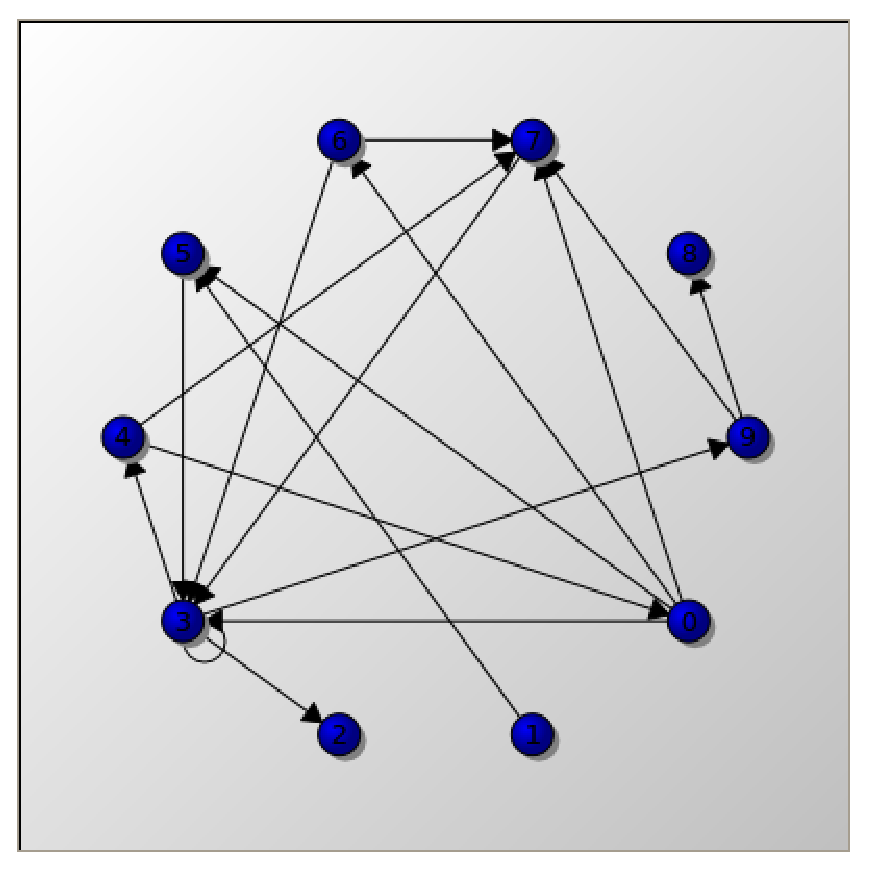
\includegraphics[scale=0.4]{graph_circle.eps}
				\end{center}
				\caption{Représentation d'un graphe disposé sur un cercle}
				\label{img_graphe_circle}
			\end{figure}
			
			\begin{figure}[htbp]
				\begin{center}
					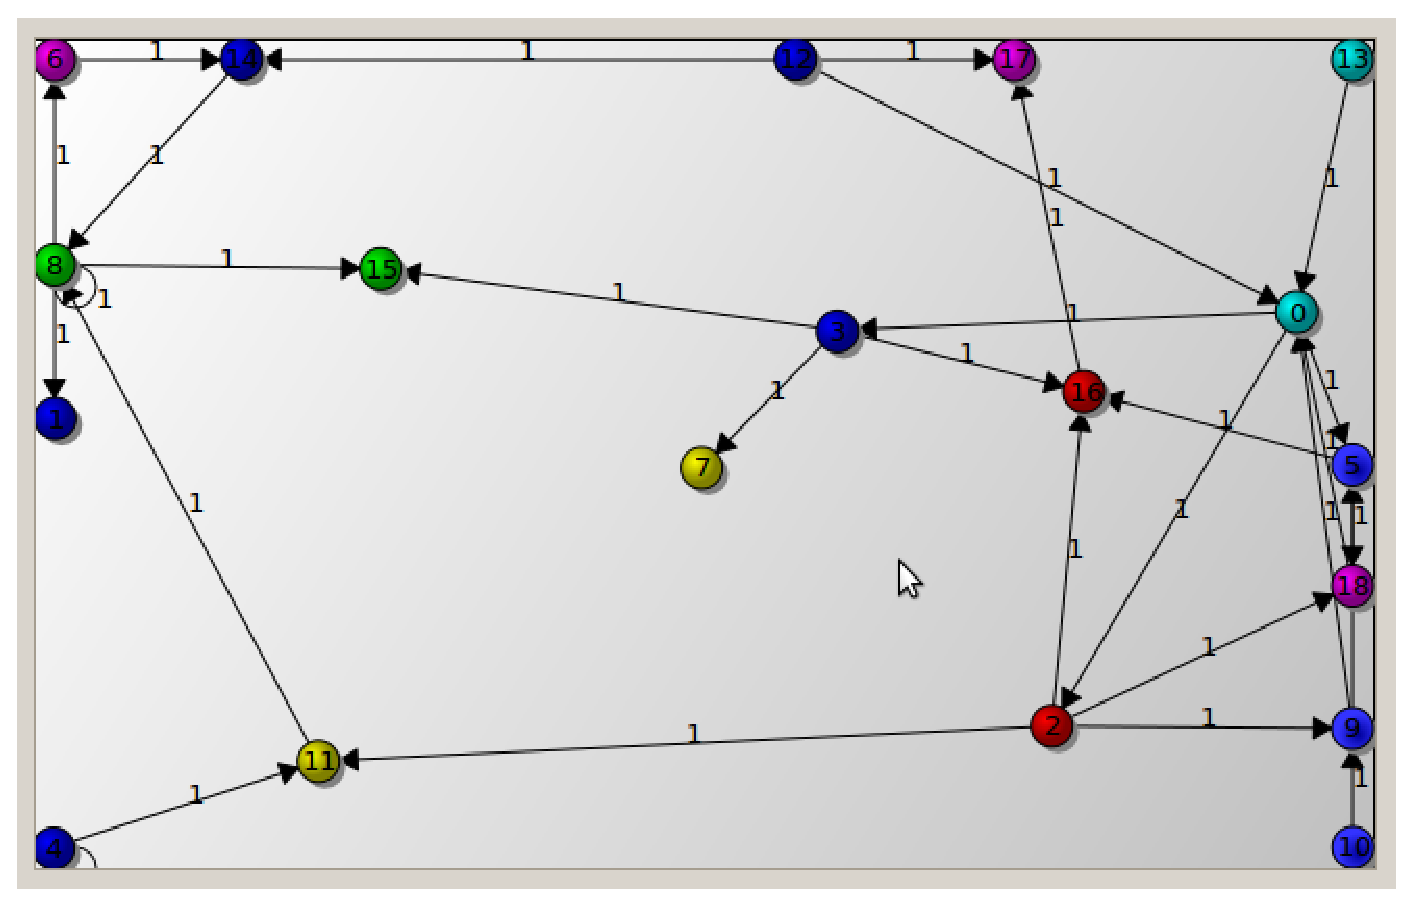
\includegraphics[width=\linewidth]{graph.eps}
				\end{center}
				\caption{Représentation d'un graphe}
				\label{img_graphe}
			\end{figure}
			
		\newpage
		\subsection{Fonctionnalités proposées}
			Le logiciel propose différentes fonctionnalités. Ces fonctionnalités ont donc du être facilement accessibles au niveau de l'interface graphique. Pour ce faire, nous avons utilisé toutes sortes de composants graphiques telles que des barres d'outils, des barres de menus ou des boites à outils permettant d'accéder aux fonctionnalités suivantes :
			\begin{itemize}
				\item \textbf{Création d'un graphe} : Grâce à cette fonctionnalité il est possible de créer ses propres graphes à l'aide de l'interface graphique. Pour cela, il suffit de double cliquer pour ajouter un n\oe ud. Pour ajouter des arcs, il suffit de cliquer une première fois sur la source de l'arc, et une deuxième fois sur la destination de l'arc. \\
				Accessible via le menu (Fig. \ref{img_barre_menu}) Fichier $\rightarrow$ Nouveau graphe ou bien via la première icône de la barre d'outils (Fig. \ref{img_barre_outil}).
				\item \textbf{Génération de graphes aléatoires }: Un graphe peut être généré de façon aléatoire. Ce graphe sera constitué d'un ensemble de n\oe uds allant de 0 à $n$ avec $n <= 20$ et d'un ensemble d'arcs compris entre 0 et $n²$.\\
				Accessible via le menu (Fig. \ref{img_barre_menu}) Fichier $\rightarrow$ Générer un graphe ou bien via la deuxième icône de la barre d'outils (Fig. \ref{img_barre_outil}).
				\item \textbf{Exportation et importation de graphe }à partir d'une librairie de graphe ou bien d'un fichier : Le logiciel permet la sauvegarde et l'ouverture de graphes. Grâce à cela, il est donc possible de charger des graphes présents dans une librairie de graphes fournis avec le logiciel, ou bien de charger un graphe à partir d'un fichier. Il est également possible de sauvegarder nos graphes préférés en mémorisant l'état de chacun de ses sommets et de ses arcs (si un algorithme est en cours d'exécution sur ce graphe, l'état de l'algorithme ne sera pas sauvegardé).
				Accessible via le menu Fichier (Fig. \ref{img_barre_menu}) ou bien via la deuxième partie de la barre d'outils (Fig. \ref{img_barre_outil}).
				\item \textbf{Ajout et modification de n\oe uds et d'arcs }: Comme pour la création d'un graphe, il est possible de modifier un graphe en lui ajoutant de nouveaux n\oe uds ou de nouveaux arcs ou bien en modifiant ceux-ci sur n'importe quel type de graphe (provenant de la libraire de graphes, d'un graphe importé ou bien d'un graphe créé par l'utilisateur).\\
				Accessible via la scène graphique (Fig. \ref{img_scene_graphique}).
				\item \textbf{Type d'affichage du graphe }: Cette fonctionnalité permet de régler différents paramètres concernant la représentation du graphe comme l'affichage des valeurs des arcs ou bien l'animation du graphe, ce qui permet de faire bouger le graphe pour le rendre le plus clair possible.\\
				Accessible via la boite d'outils (Fig. \ref{img_boite_outil}).
				\item \textbf{Sélection d'algorithmes }: Le logiciel permet d'exécuter différents algorithmes en rapport avec les graphes. Il est donc possible de choisir un algorithme parmi la liste des algorithmes fournis par le logiciel et de l'exécuter.\\
				Accessible via la dernière partie de la barre d'outils (Fig. \ref{img_barre_outil}).
				\item \textbf{Lancement d'algorithmes }: Permet de lancer l'algorithme sélectionné dans la barre d'outils (Fig. \ref{img_barre_outil}) et permet de visualiser son déroulement sur la scène graphique (Fig. \ref{img_scene_graphique}).
				Accessible via la boite d'outils (Fig. \ref{img_boite_outil}) ou bien par le menu Algorithme (Fig. \ref{img_barre_menu}).
				\item \textbf{Type d'interaction avec l'algorithme }: Il est possible d'interagir avec un algorithme lors de son déroulement. Ce type d'interaction peut varier. L'utilisateur peut cliquer sur les n\oe uds qu'il veut ou bien laisser l'ordinateur choisir. Les choix de l'ordinateur sont de différents types : 
				\begin{itemize}
					\item Fifo, qui permet de sélectionner le premier n\oe ud de la liste des n\oe uds disponible
					\item Lifo, qui choisit le dernier n\oe ud
					\item Aléatoire, qui choisit un n\oe ud de façon aléatoire parmi les n\oe uds disponibles.
				\end{itemize}
				Accessible via la boite d'outils (Fig. \ref{img_boite_outil}).
				\item \textbf{Vitesse de défilement de l'algorithme }: Lorsque le type d'interaction permet à l'ordinateur de choisir ses propres n\oe uds. Il est nécessaire de pouvoir voir les choix de l'algorithme. Pour ce faire, on peut indiquer à l'algorithme le temps qu'il doit attendre avant de prendre une nouvelle décision.\\
				Accessible via la boite d'outils (Fig. \ref{img_boite_outil}).
			\end{itemize}
		
		\newpage
			\begin{figure}[h!]
				\begin{minipage}[b]{1\linewidth}
					\centering
					
\includegraphics[scale=0.64]{menuBar.eps}
					\caption{Barre de menu}
					\label{img_barre_menu}
					\vspace{.5cm}
				\end{minipage}
				\begin{minipage}[b]{1\linewidth}
					\centering
					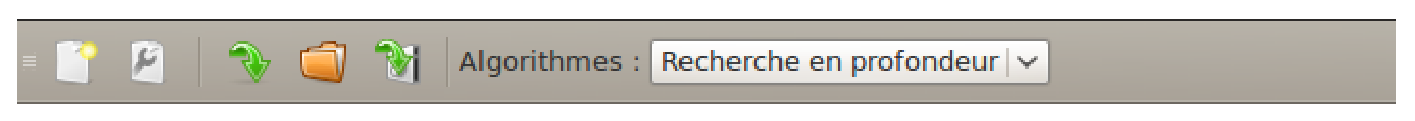
\includegraphics[scale=0.64]{toolBar.eps}
					\caption{Barre d'outils}
					\label{img_barre_outil}
					\vspace{.5cm}
				\end{minipage}
				\begin{minipage}[b]{0.5\linewidth}
					\centering 
					
\includegraphics[scale=0.6]{graphicView.eps}
					\caption{Scène graphique}
					\label{img_scene_graphique}
				\end{minipage}\hfill
				\begin{minipage}[b]{0.5\linewidth}   
					\centering 
					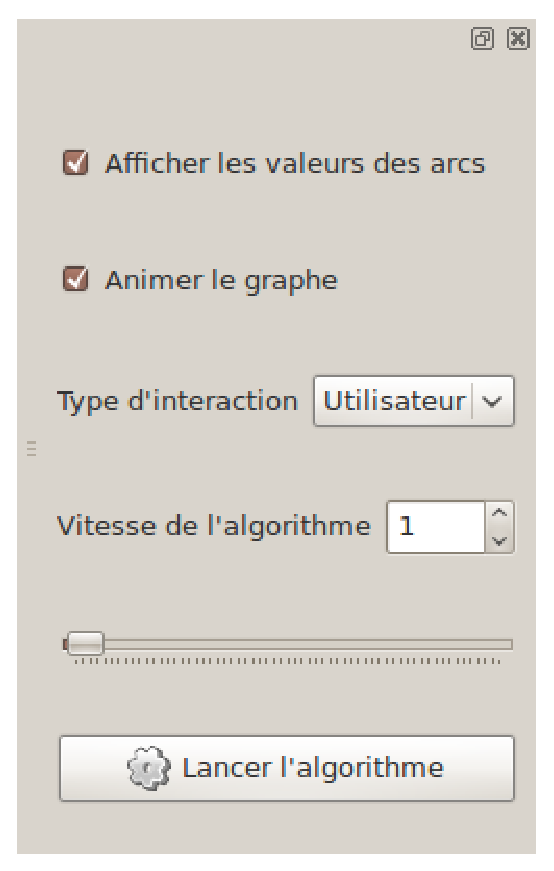
\includegraphics[scale=0.6]{toolBox.eps}
					\caption{Boite à outils}
					\label{img_boite_outil}
				\end{minipage}
			\end{figure}
			
	\newpage
	\section{Interaction entre l'interface graphique et l'algorithme}
		Pour donner un peu plus de dynamisme au logiciel, l'utilisateur devait pouvoir interagir avec l'algorithme qu'il avait lancé. Cette fonctionnalité permet d'indiquer à l'algorithme les n\oe uds par lesquels il doit passer, le tout en ayant un aperçu, au cours de l'algorithme, des choix que l'on a indiqué à l'algorithme et des opérations que celui-ci a effectuées. Pour cela, nous avons donc d'abord utilisé le pattern de conception observateur, qui permet de mettre à jour, dans notre cas, des composants graphiques dès qu'on en a besoin et ensuite temps des threads permettant l'utilisation de l'algorithme et de l'interface graphique en parallèle.
		\subsection{Le pattern Observateur}
			\begin{figure}[htbp]
				\begin{center}
					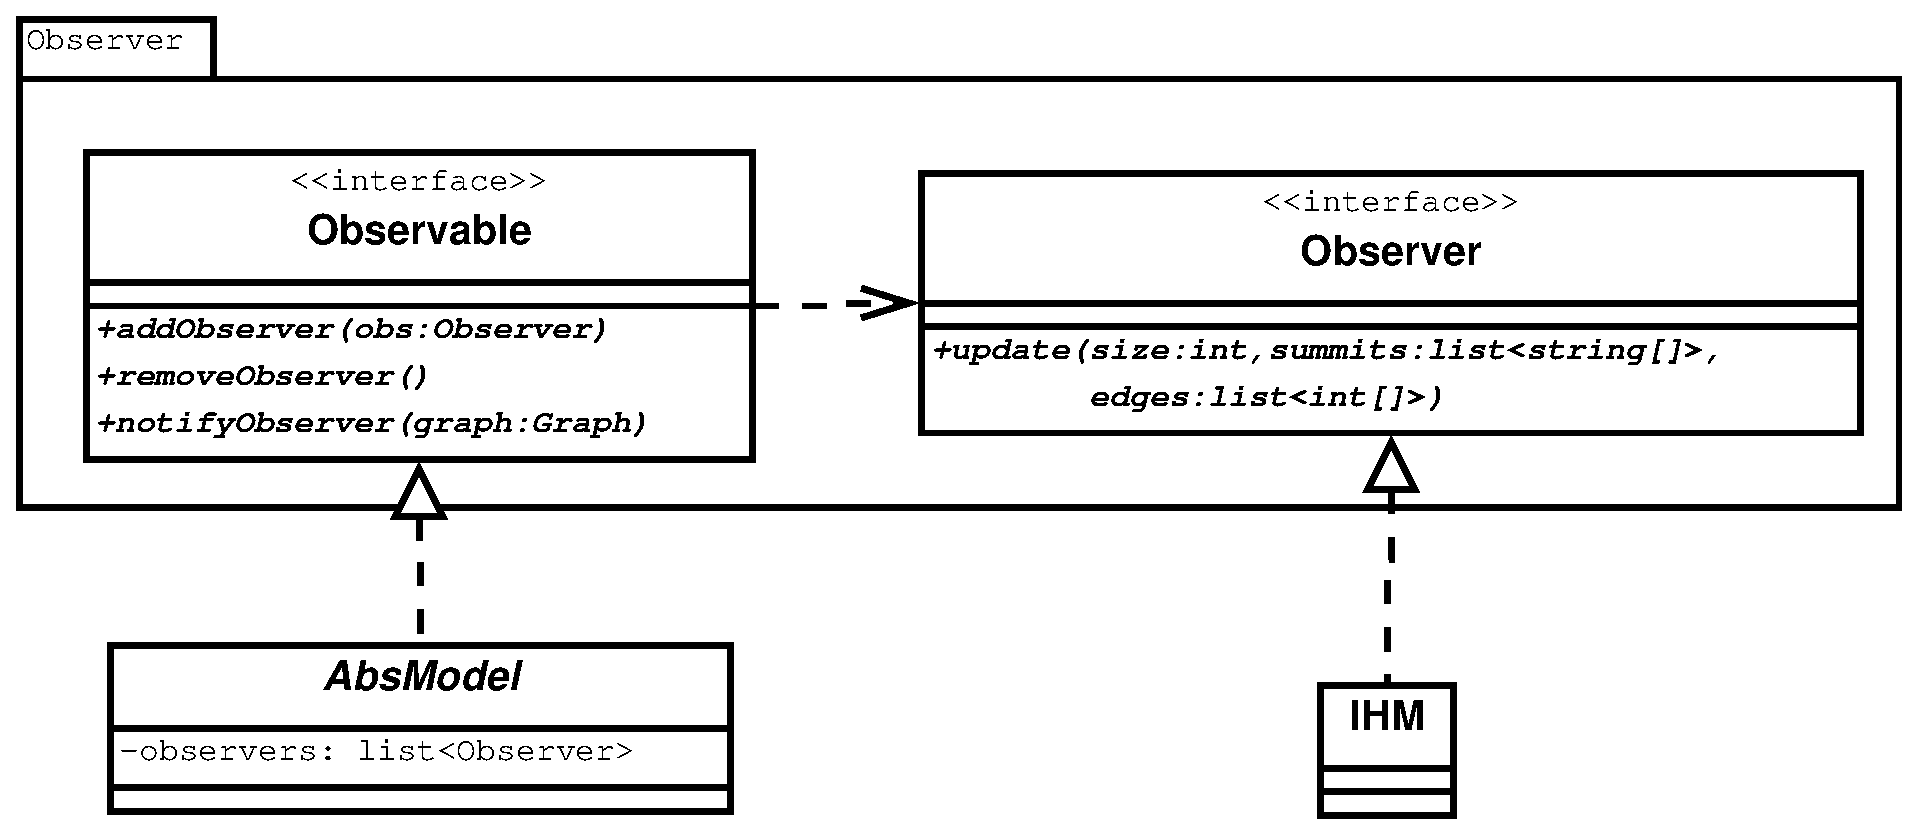
\includegraphics[scale=0.4]{observer.eps}
				\end{center}
				\caption{Pattern observateur implémenté}
				\label{img_observer}
			\end{figure}
			Comme on peut le voir à l'aide du diagramme UML (Fig. \ref{img_observer}), dans cette implémentation du pattern observateur que nous avons utilisé, lorsque nous modifions notre graphe, cette modification sera suivie de l'appel de la fonction \textit{notifyObserver(graph:Graph)}, dans laquelle la paramètre fourni sera le graphe avec ses nouvelles modifications. Cette fonction va donc parcourir l'ensemble des \textit{observers} (qui sont en réalité des composants de notre fenêtre, voire la fenêtre elle-même) et leur envoyer le nouvel état du graphe. Une fois ces informations reçues, chaque \textit{observer} va traiter ces informations en fonction de ce dont elle a besoin. Pour ce projet, un seul \textit{observer} existe pour l'instant, qui se trouve être la représentation graphique du graphe (Fig. \ref{img_scene_graphique}). 
			A l'aide de ce procédé, l'utilisateur peut maintenant effectuer des modifications sur le graphe et avoir une représentation de cette modification. 
			
			En quoi ceci permet t-il d'interagir avec l'algorithme?
			
			Lors du déroulement de l'algorithme, celui-ci va proposer une liste de n\oe uds que l'utilisateur pourra choisir. Pour ce faire, l'algorithme va affecter à ces n\oe uds un état prédéfini pour la sélection. Lorsque l'interface graphique rencontre un n\oe ud avec cet état là, elle permet le clic sur ce n\oe ud, ce qui prévient l'algorithme que le n\oe ud en question a été choisi et l'algorithme peut donc continuer.
			
		\subsection{Utilisation de Threads}
			Lorsque l'algorithme propose une liste de n\oe uds à l'utilisateur, celui-ci doit attendre le choix de l'utilisateur. Ceci crée un problème. En effet, étant donné que l'algorithme a été lancé par le biais de l'interface graphique et que cet algorithme est maintenant en attente, cela implique donc que l'interface graphique est également en attente et ne peut donc pas gérer les évènements de clics, par exemple pour choisir un n\oe ud. Il est donc impossible de pouvoir choisir un n\oe ud que propose l'algorithme, car tant que l'algorithme n'est pas terminé, l'interface graphique reste figée. Pour régler ce problème, il serait donc intéressant de pouvoir lancer l'algorithme en parallèle de l'interface graphique et que les deux processus puissent s'exécuter séparément, mais tout en gardant une communication entre eux. Nous aurions pu lancer l'algorithme dans un nouveau programme, mais nous aurions perdu la communication entre l'interface graphique et l'algorithme. Ceci n'était donc pas une bonne solution.
			
			Après avoir bien cerné le problème, nous avons donc eu l'idée de threader notre programme. En effet, si nous lançons un algorithme dans un nouveau thread, cela aurait pour conséquence d'exécuter en parallèle notre algorithme et notre interface graphique et donc, lorsque l'algorithme attendrait que l'utilisateur choisisse un n\oe ud, il n'empêcherait pas la fenêtre de se mettre à jour et de gérer ses évènements. L'utilisateur aura donc la possibilité d'effectuer diverses opérations sur la fenêtre, comme par exemple, choisir un n\oe ud. 

	A cet instant le logiciel était en mesure de lancer un algorithme, de mettre en attente celui-ci tout en ayant une interface graphique toujours fonctionnelle. Cependant, comment faire pour que l'algorithme sorte de son état d'attente? Pour cela, nous avons donc eu l'idée d'affecter un état à l'algorithme en fonction du choix de l'utilisateur. Il existe deux types d'états :
		\begin{itemize}
			\item En attente lorsque l'utilisateur n'a pas encore choisi de n\oe ud.
			\item Actif lorsque l'utilisateur a choisi un n\oe ud et cet état contient également la valeur du n\oe ud sélectionné.
		\end{itemize}
		A l'aide de cela, il a été facile de gérer l'attente de l'algorithme car celui-ci entre dans une boucle qui le fait attendre tant que l'état de l'algorithme n'est pas actif, et le changement d'état se fait lorsque l'utilisateur clique sur un n\oe ud. Cette technique se rapproche de l'utilisation de sémaphores permettant de gérer l'état d'un thread, mais avec, ici, en plus, la valeur désirée pour que l'algorithme puisse continuer.
		
		Grâce à cela notre utilisateur est donc en mesure de lancer un algorithme, puis d'indiquer à l'algorithme les n\oe uds par lesquels il doit passer.
		
		Grâce à l'utilisation de ce thread, il est donc également possible de modifier en plus de l'état du graphe, les caractéristiques de l'algorithme, comme par exemple, le type d'interaction ou bien la vitesse de défilement de celui-ci (cf Interface Graphique $>$ Fonctionnalités proposée) pendant son déroulement.
	
	\newpage
	\section{Discussions}
		Maintenant que ce rapport arrive à sa fin, prendre un peu de recule sur le projet est essentiel. Concernant les objectifs du cahier des charges, ceux-ci ont été remplis, certains avec un peu plus de difficultés que d'autres, mais cela n'a pu être que bénéfique. Grâce à ces quelques difficultés, nous avons pu apprendre à maitriser de nouvelles techniques et outils. Cela nous a donc été grandement profitable. Nous avons réussi à faire un logiciel assez évolutif, dans lequel il est possible de rajouter des structures de graphe et des algorithmes, facilement.
		
		Le déroulement du projet s'est assez bien passé, le planning prévisionnel était bien fait. En effet, celui-ci était en adéquation avec le déroulement du projet.
		
		Concernant d'éventuelles améliorations, plusieurs peuvent être envisagées. Dans un premier temps, développer plus d'algorithmes afin d'avoir une vraie librairie d'algorithmes contenant une dizaine d'algorithmes différents. Nous pourrions également améliorer l'interface graphique qui est assez simpliste, mais fonctionnelle. La grosse amélioration possible concerne la configuration de l'algorithme comme le type d'interaction avec l'algorithme ou bien la vitesse de celui-ci. En effet, le type d'interaction  propose différents choix (Utilisateur, Aléatoire, Fifo, Lifo) seulement, suivant l'algorithme développé, celui-ci ne propose pas forcément un choix donc cet outil peut \^etre inutile. Il serait donc envisageable d'afficher ce composant uniquement en fonction de l'algorithme choisi. De même, pour le choix de la vitesse, cette vitesse est exprimée en secondes. Suivant l'utilisation qu'on fait de ce logiciel, il peut être intéressant que la vitesse soit exprimée dans une, voire plusieurs autres unités de temps. Enfin, il serai bon de rajouter la sauvegarde de la configuration du logiciel afin que l'utilisateur puisse retrouver les choix qu'il a fait lors de la dernière utilisation du logiciel.

		Concernant la création du graphe, celle-ci se fait uniquement à l'aide de clics au sein de l'interface graphique avec un double clic pour créer un n\oe ud et deux clics successifs entre deux n\oe uds pour créer un arc. Cette méthode peut déplaire à certains utilisateurs.
		
		 Tout cela n'était pas précisé dans le cahier des charges, de ce fait, seul un test auprès de différents utilisateurs du logiciel pourrait permettre de les définir de façon plus précise.
		
	\newpage
	\section{Conclusion}
		Pour conclure, ce projet a été très intéressant. Tout d'abord car il nous a permis de mettre en pratique certaines connaissances découvertes lors de nos cours et plus particulièrement concernant les design pattern tel que la programmation en couches et l'utilisation du pattern M.V.C. ainsi que des fabriques abstraites. Ce projet nous a également permis de pouvoir planifier nos tâches et de voir que cela n'était pas forcément aisé de diriger un projet. Concernant l'équipe, cela s'est, hélas, assez mal passé. En effet, suite à très peu d'investissement dans le projet de la part de mon binôme, nous avons été contraint de nous séparer. Ceci à donc créer quelques problèmes, le premier étant bien sûr la charge de travail. En effet, le planning était fait pour deux personnes, après cette séparation je me suis retrouvé seul pour faire le projet.
		
		~\\
		\indent Dans l'ensemble ce projet a apporté beaucoup, notamment l'apprentissage du chargement dynamique d'objets en C++, qui n'est pas une mince affaire, la création d'une fabrique permettant notamment la sauvegarde et l'importation de graphes en XML. De plus, le développement s'est fait en C++, ce qui nous a permis d'apprendre à maitriser un peu plus ce langage, ainsi que la librairie graphique Qt qui est une librairie beaucoup utilisée. 
		
		~\\
		\indent Au final, ce projet a été très bénéfique, que ce soit d'un point de vue programmation, organisation ou même réflexion. Il nous a permis de faire diverses découvertes, le sujet était plaisant et le fait de savoir que ce logiciel pourrait être utilisé par la suite a été très motivant.
	
	\newpage
	\section{Annexes}
		\subsection{Diagramme de classe}
			\subsubsection*{Modèle}
				\begin{figure}[htbp]
					\begin{center}
						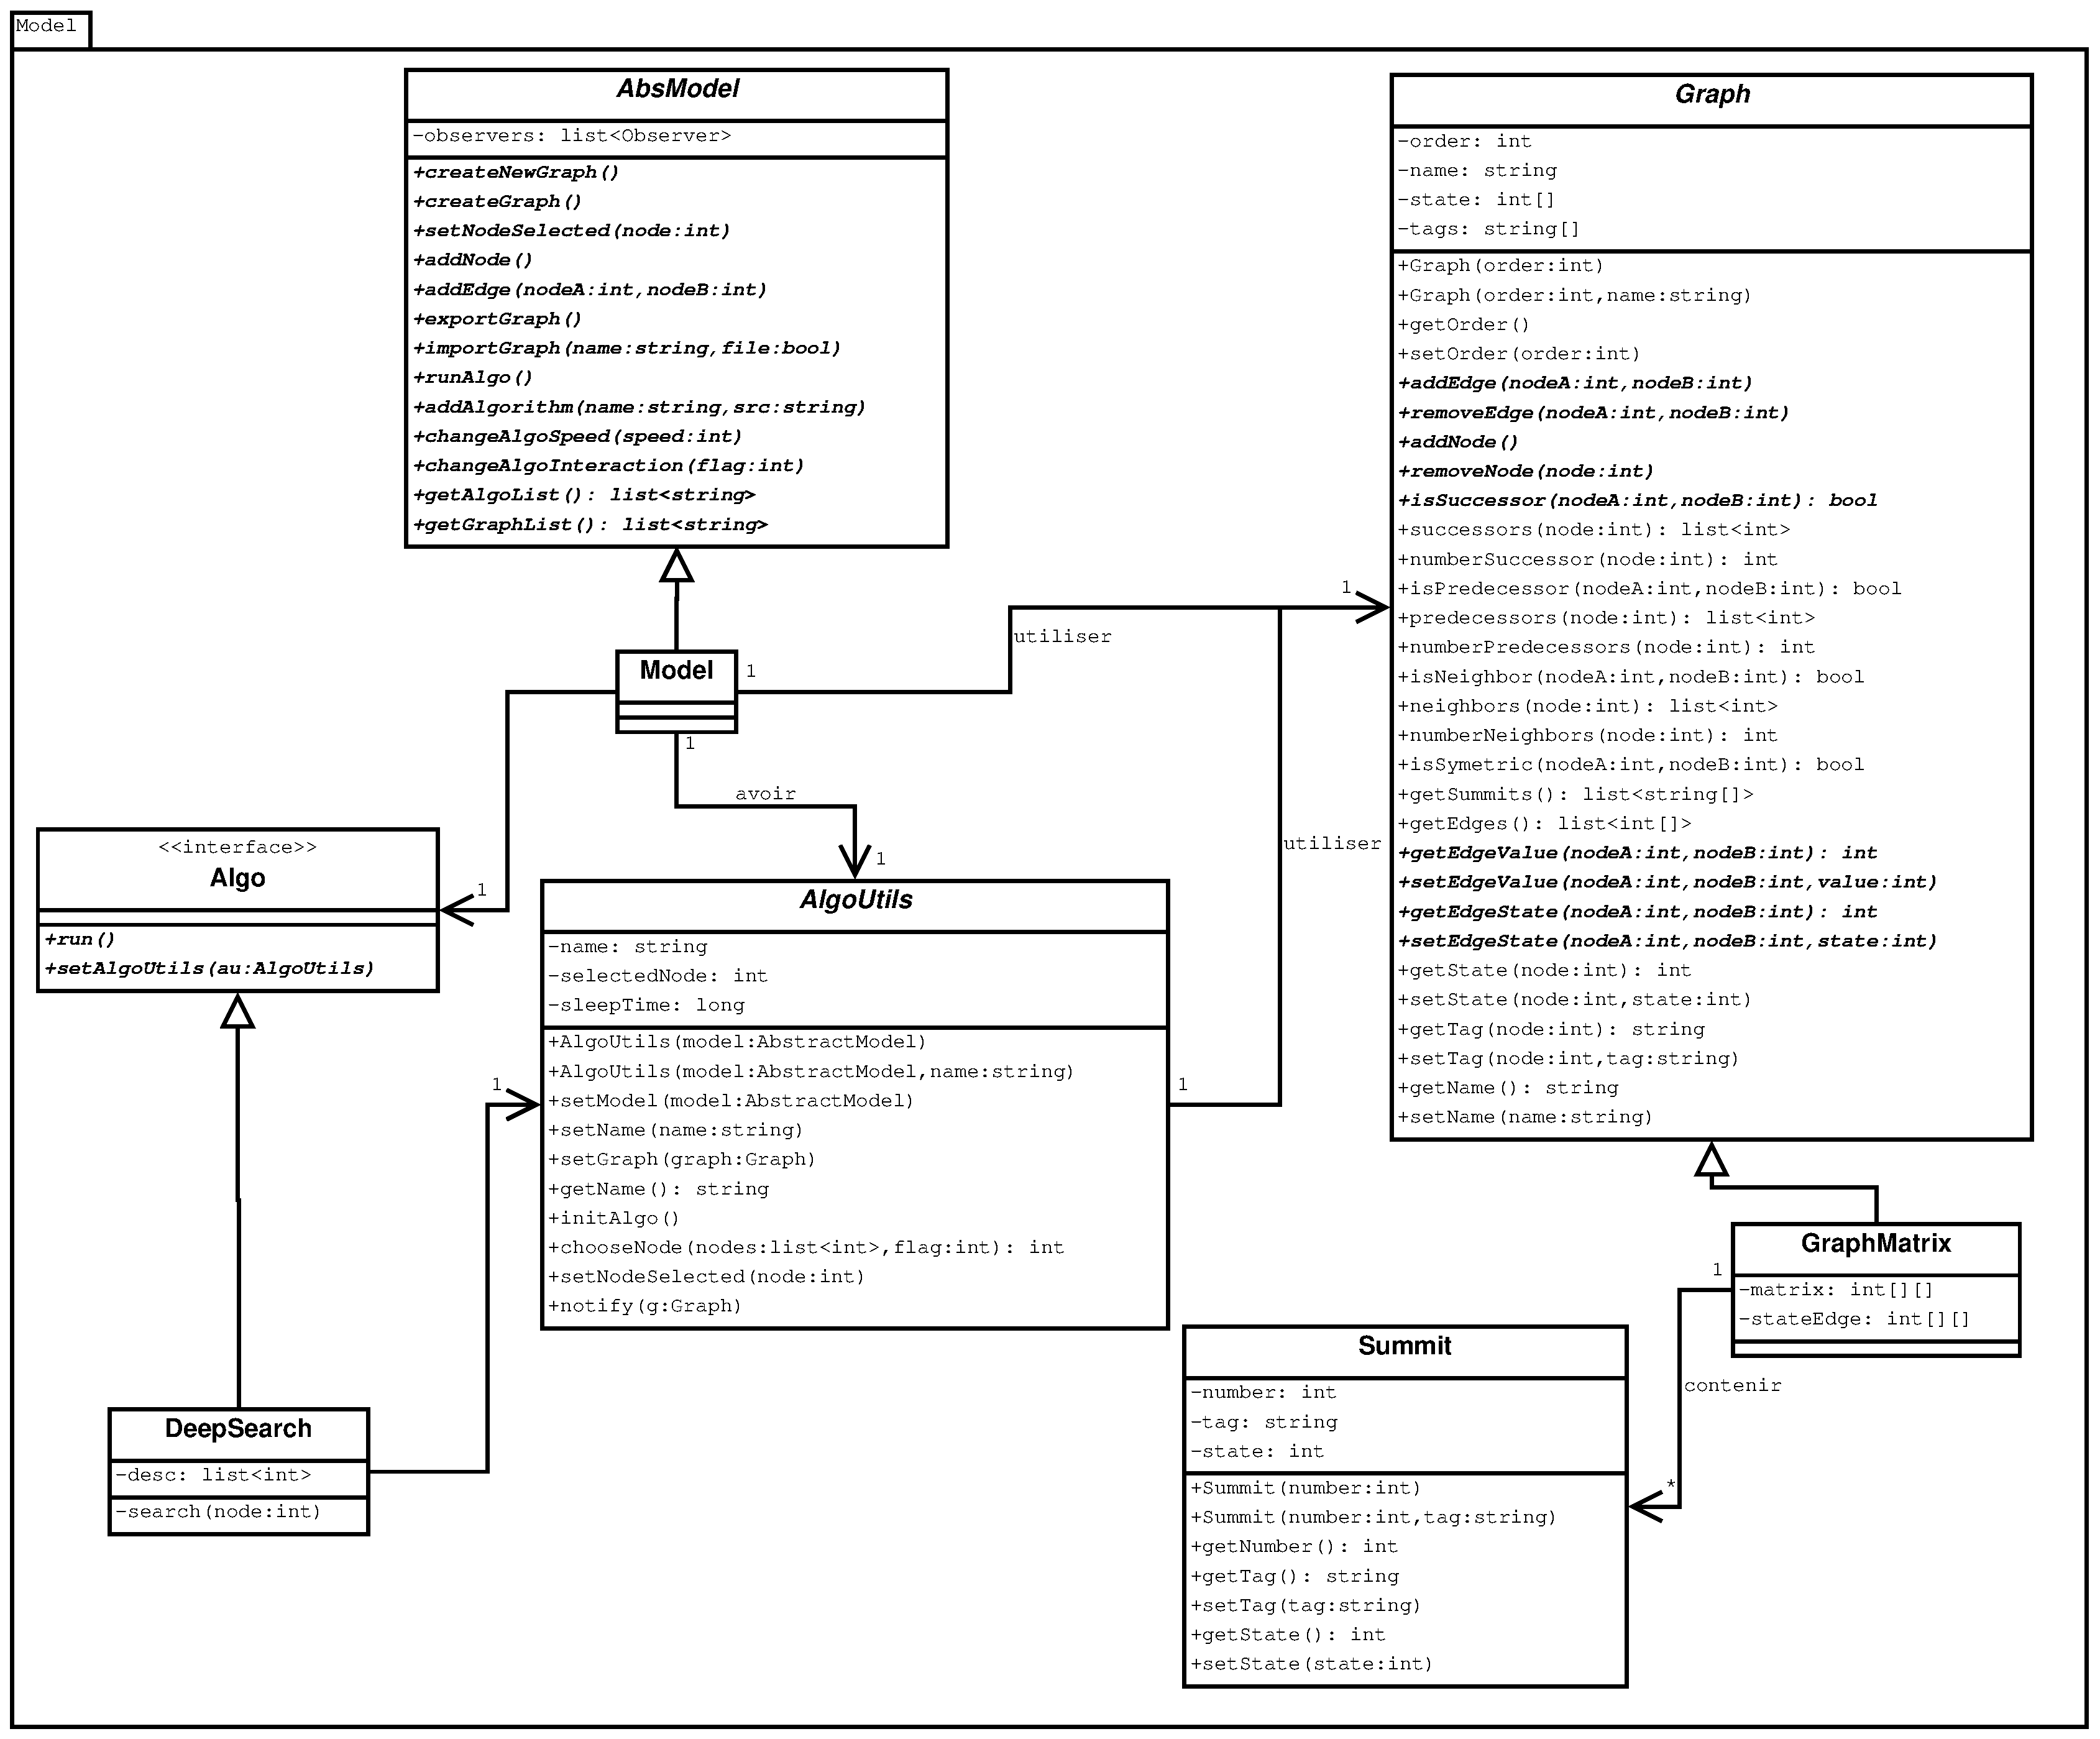
\includegraphics[width=\linewidth]{class_model.eps}
					\end{center}
					\caption{Package modèle}
					\label{img_class_model}
				\end{figure}
				\newpage
			\subsubsection*{Sérialisation}
				\begin{figure}[htbp]
					\begin{center}
						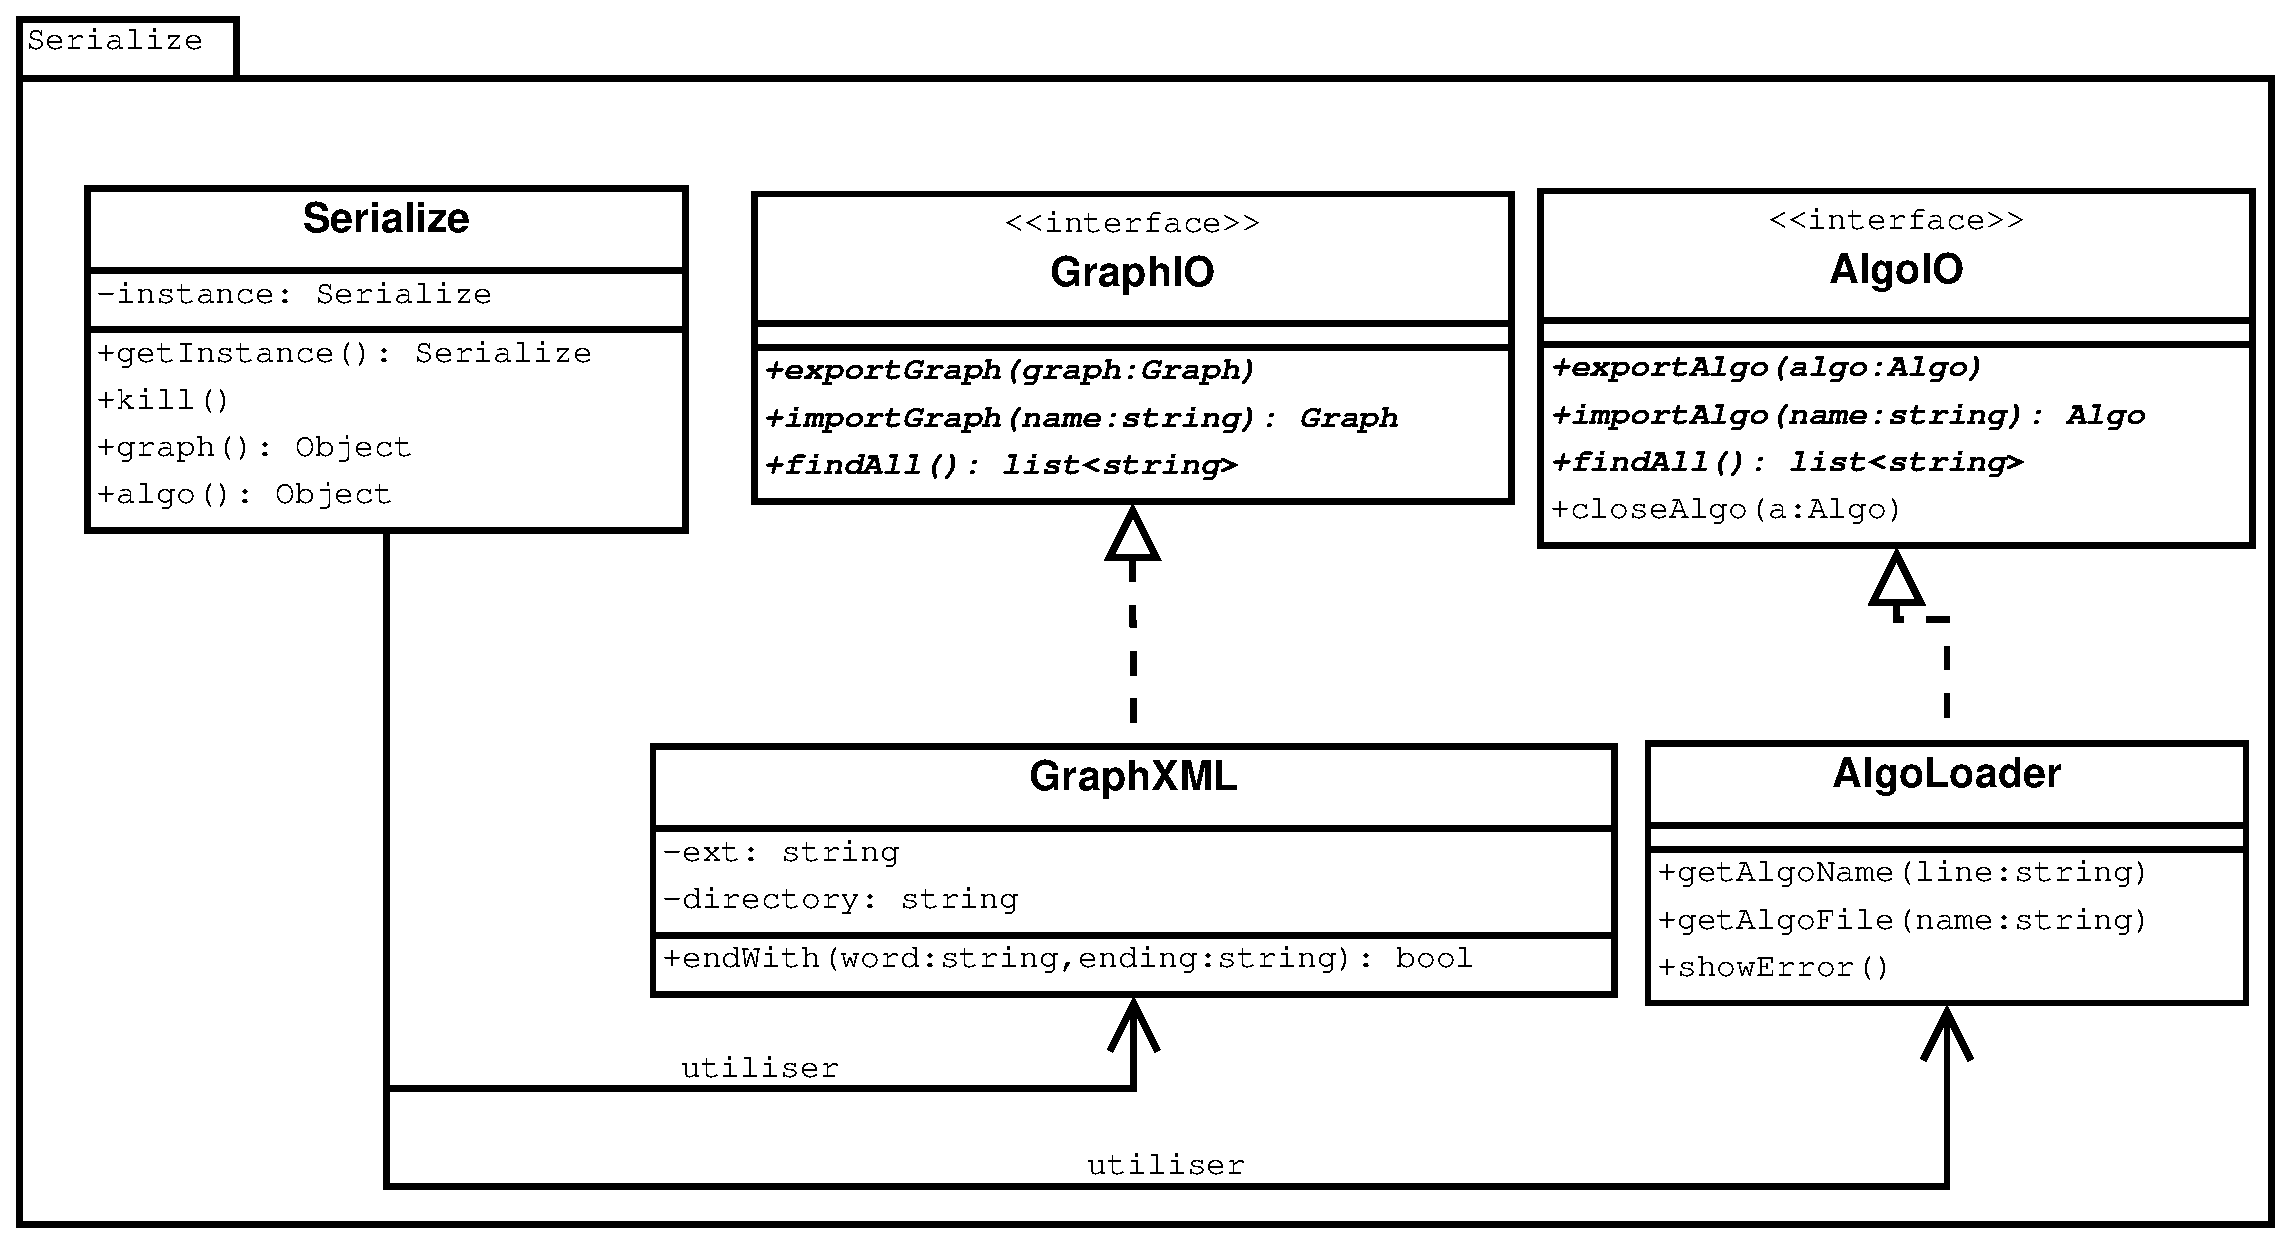
\includegraphics[width=\linewidth]{class_serialize.eps}
					\end{center}
					\caption{Package sérialisation}
					\label{img_class_serialize}
				\end{figure}
			\subsubsection*{Contrôleur}
				\begin{figure}[htbp]
					\begin{center}
						\includegraphics[scale=.4]{class_controller.eps}
					\end{center}
					\caption{Package contrôleur}
					\label{img_class_controler}
				\end{figure}
				\newpage
			\subsubsection*{Observateur}
				\begin{figure}[htbp]
					\begin{center}
						\includegraphics[width=0.75\linewidth]{class_observer.eps}
					\end{center}
					\caption{Package observateur}
					\label{img_class_observer}
				\end{figure}
			\subsubsection*{Interface Graphique}
				\begin{figure}[htbp]
					\begin{center}
						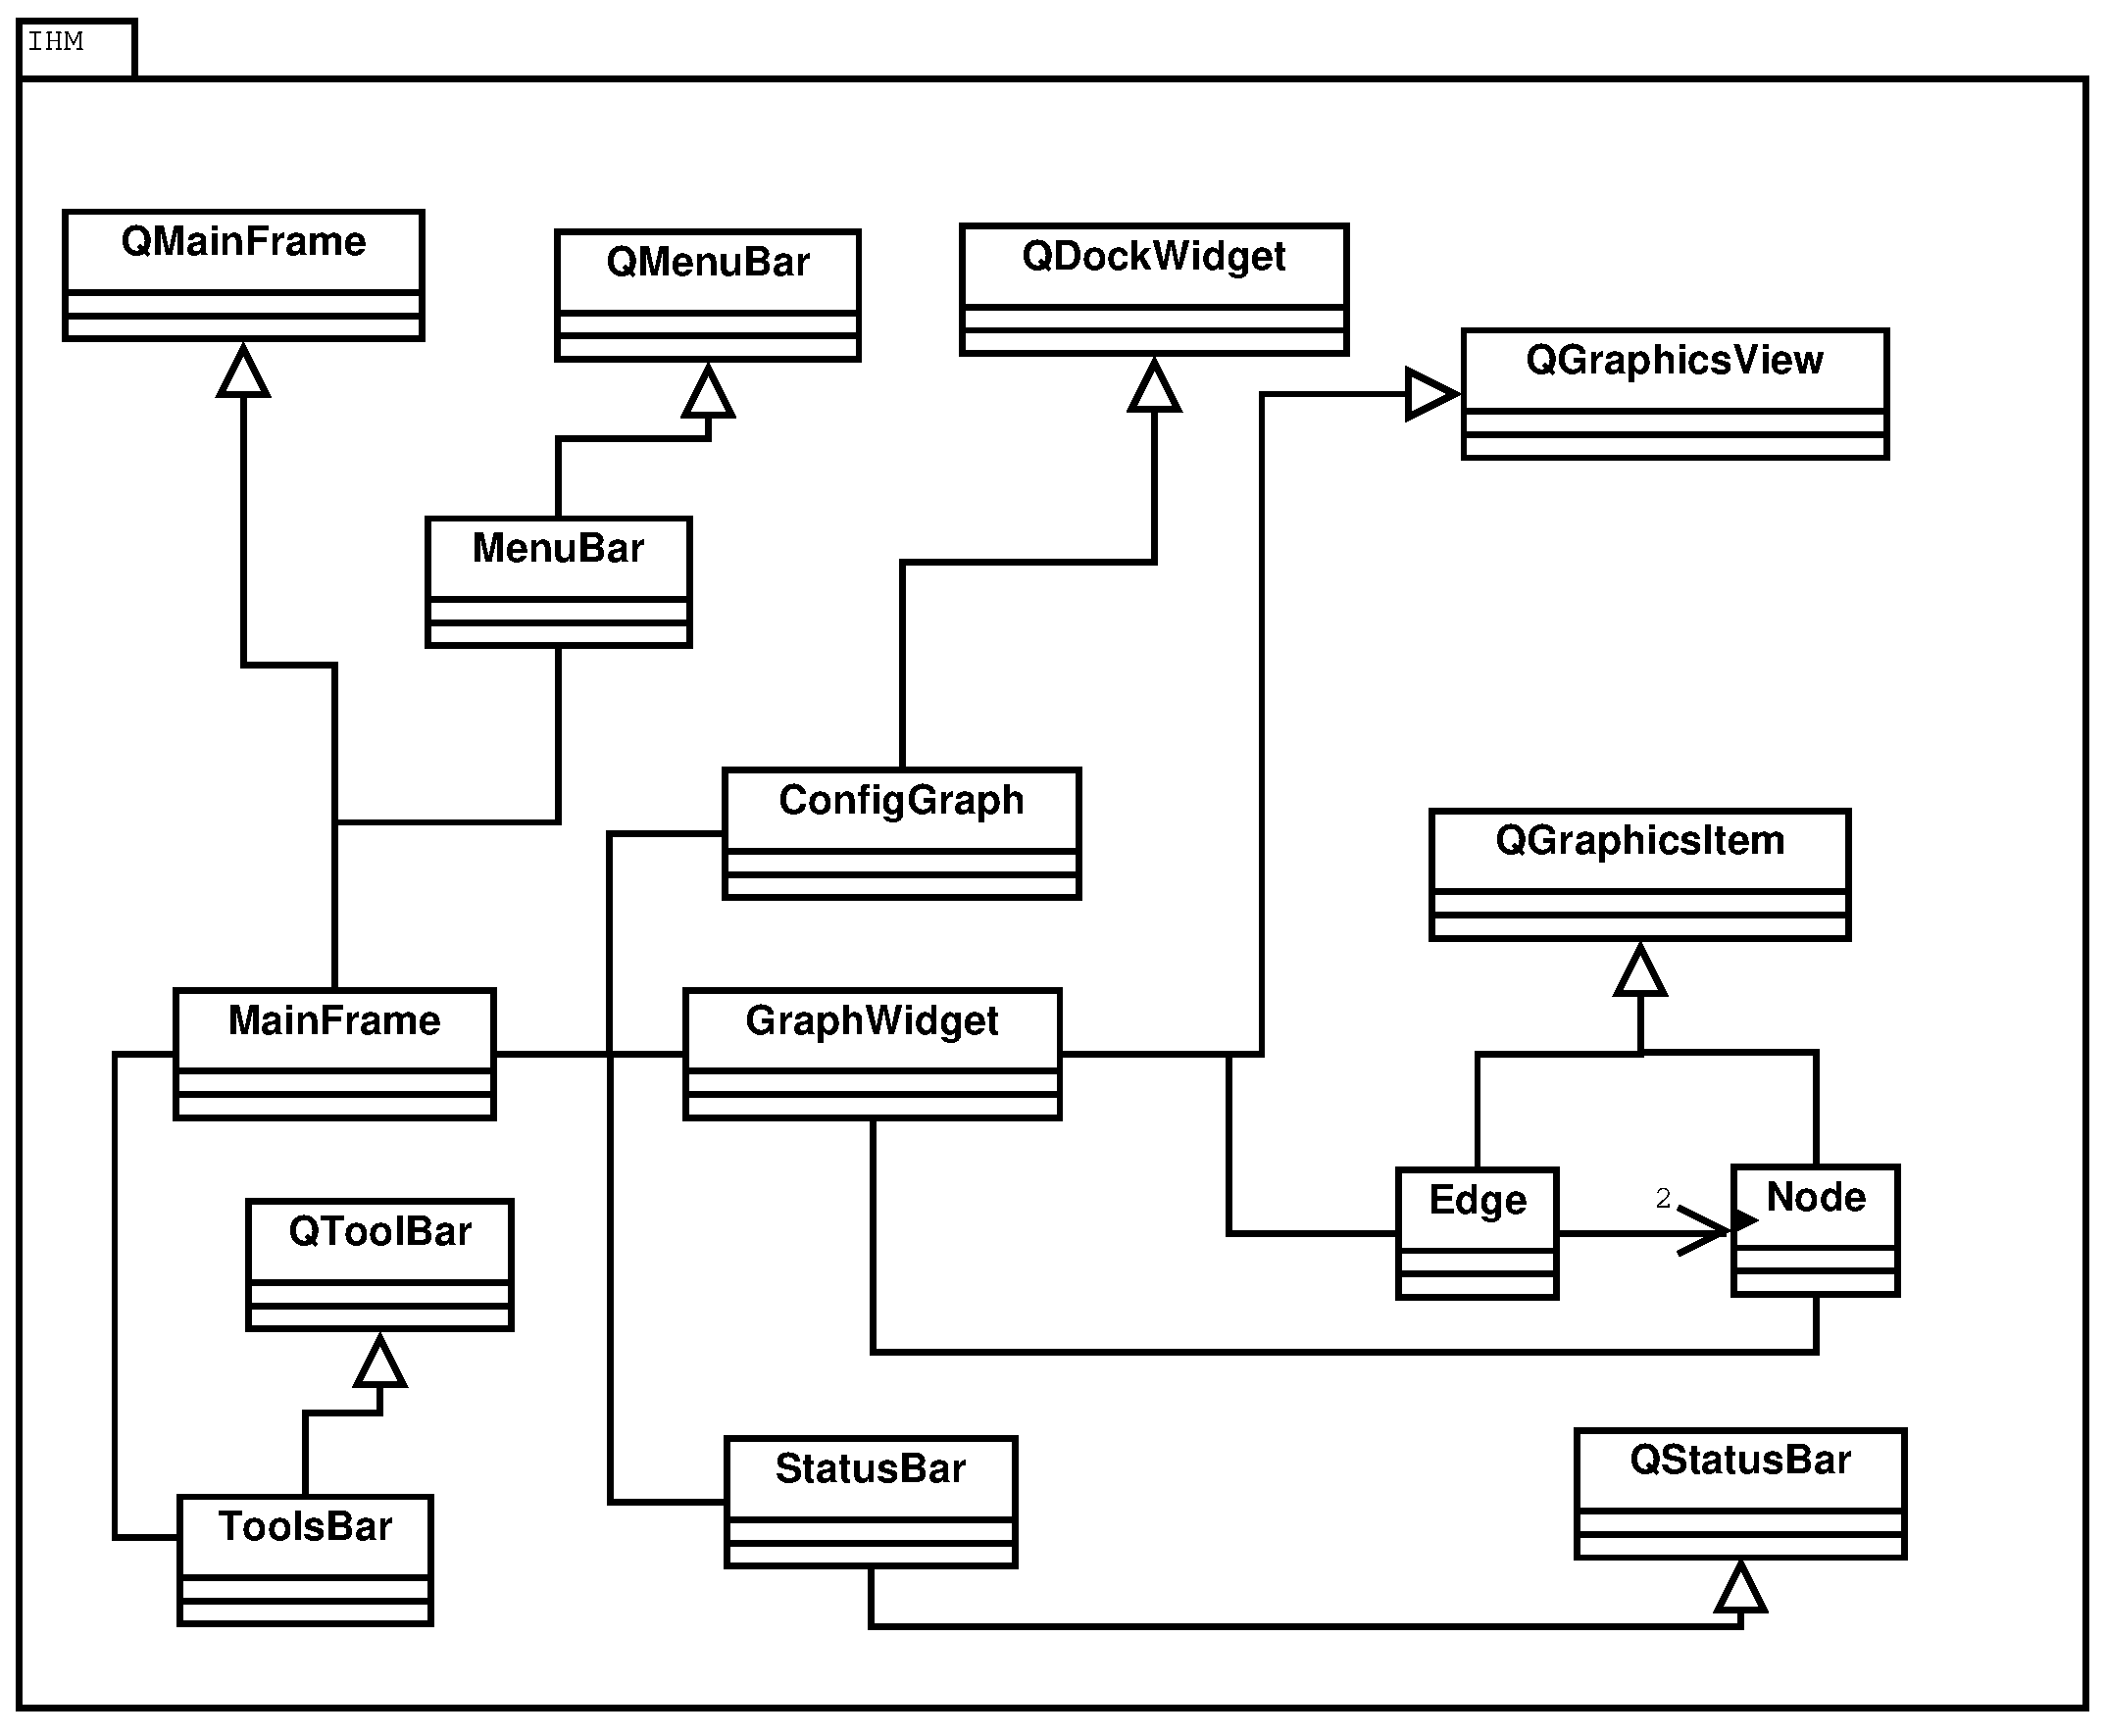
\includegraphics[width=0.75\linewidth]{class_ihm.eps}
					\end{center}
					\caption{Package interface graphique}
					\label{img_class_ihm}
				\end{figure}
		
		\newpage
		\subsection{Bibliographie et sitographie}
	
			\noindent De manière générale : \\
			\begin{itemize}
				\item \textit{www.google.fr}\\
				\item \textit{fr.wikipedia.org/}\\
				\item \textit{www.siteduzero.com/}\\
			\end{itemize}
	
			\noindent Page relative à la librairie Qt	:\\
			\begin{itemize}
				\item \textit{doc.trolltech.com/4.6/index.html}\\
			\end{itemize}
	
			\noindent Pages relatives au chargement dynamique des algorithmes : \\
			\begin{itemize}
				\item \textit{www.linux-kheops.com/doc/man/manfr/man-html-0.9/man3/dlopen.3.html}\\
				\item \textit{hiko-seijuro.developpez.com/articles/bibliotheque-dynamique/}\\
				\item \textit{en.wikipedia.org/wiki/Dynamic-link\_library}\\
				\item \textit{en.wikipedia.org/wiki/Dynamic\_loading}\\
				\item \textit{www.faqs.org/docs/Linux-mini/C++-dlopen.html}\\
			\end{itemize}
			
			\noindent Pages relatives à la sérialisation xml : \\
			\begin{itemize}
				\item \textit{www.grinninglizard.com/tinyxmldocs/index.html}\\
			\end{itemize}
		
	\newpage
	\section*{\begin{center}Resumé\end{center}} 
		
		Ce projet sous la tutelle de Mr Cogis a pour objectif de créer un logiciel pédagogique pour la compréhension d'algorithmes de graphes. Celui-ci, permettra à un utilisateur de créer ou visualiser des graphes et d'appliquer des algorithmes sur ceux-ci. Au cours de l'un de ces algorithmes, l'utilisateur aura la possibilité de choisir ses n\oe uds et de ce fait, pourra guider l'algorithme. Ces algorithmes pourront être ajoutés à la manière de greffons. Ainsi, les utilisateurs pourront développer leurs propres algorithmes et les ajouter facilement.\\
		
		Ce logiciel pourra donc servir dans divers domaines et notamment dans l'enseignement lors de l'apprentissage des graphes ou bien d'algorithmes de graphes.

	\vspace{2cm}
	
		\section*{\begin{center}Abstract\end{center}}
		
		This project under the direction of Mr Cogis aims to create an educational software to understanding graphs algorithms. This allows a user to create or view graphs and perform algorithms on them. During these algorithms, users have the opportunity to choose nodes and therefore can direct the algorithm. These algorithms can be added like plugins. The users can develop their own algorithms and add them easily.
\\

This software can be used in several domains, particularly in education to learn graph or graph algorithms.

\thispagestyle{empty}
\end{document}